\section{Algorithm}
\label{app:algorithm}

\begin{figure}[h]
\small
\begin{minipage}{0.96\linewidth}
\textbf{Algorithm 1: QKSieve for one request}\\[2pt]
\textbf{Input:} dense prompt; exact GPU-resident KV; head dimension
$d=128$; Key stride 32; Query-tail length 8; rate 240 bits.\\
\textbf{After dense prefill:}\\
1.\ For each layer and KV head, form $C_k$ from stride-32 post-RoPE Keys.\\
2.\ Group all mapped GQA Query heads and form $C_q$ from the final eight
prompt positions; apply \cref{eq:q-shrink}.\\
3.\ Compute \cref{eq:qk-svd,eq:qk-factors} and project sampled Keys and
Queries.\\
4.\ Evaluate \cref{eq:band-qmse} for each band and bit level; solve
\cref{eq:qmse-allocation} exactly and freeze the allocation.\\
5.\ Project all prompt Keys in chunks and write the packed mixed-bit index.\\
\textbf{For each generated token:}\\
6.\ Project and INT8-quantize every Query head.\\
7.\ Scan the complete packed index and take approximate-score top-$B(N)$.\\
8.\ Gather original FP16 K/V at those positions and compute exact sparse
QK--softmax--AV.\\
9.\ Append the new exact K/V and its projected packed-Key entry.\\
\textbf{Output:} the ordinary decoder hidden state and updated exact KV plus
index.
\end{minipage}
\end{figure}

\section{Extended Theoretical Statements}
\label{app:analysis-statements}

We separate exact algebraic properties from assumptions used to make the
mixed-bit objective separable.  Full proofs are in \cref{app:proofs}.

\subsection{Exactness and balanced score geometry}

\paragraph{Proposition 1 (exact biorthogonal score preservation).}
Let $\widetilde C_q,C_k\in\R^{d\times d}$ be positive definite and let
$A,D$ be defined by \cref{eq:qk-svd,eq:qk-factors}.
Then
\begin{equation}
 AD^\top=I.
 \label{eq:prop-biorthogonal}
\end{equation}
Consequently, for every $q,k\in\R^d$, not only for calibration samples,
\begin{equation}
 (A^\top q)^\top(D^\top k)=q^\top k.
 \label{eq:prop-score-exact}
\end{equation}
Thus \method's transform is not a low-rank approximation and adds no
full-precision score error.

\paragraph{Proposition 2 (simultaneous second-moment balance).}
Under the same conditions,
\begin{equation}
 A^\top\widetilde C_qA=D^\top C_kD=\Sigma.
 \label{eq:prop-cov-balance}
\end{equation}
If transformed Queries and Keys are paired independently according to these
second moments, their expected squared dot product is
\begin{equation}
 \mathbb E[({q'}^\top k')^2]=\tr(\Sigma^2)
 =\sum_{\ell=1}^{d}\sigma_\ell^2.
 \label{eq:score-energy}
\end{equation}
Therefore the singular order exposes joint score energy: retaining the first
$r$ unquantized coordinates leaves expected tail score energy
$\sum_{\ell>r}\sigma_\ell^2$ under the construction moments.
With shrinkage and the spectral floor,
\cref{eq:prop-cov-balance} holds exactly for the construction moments
$\widetilde C_q$ and $C_k$, while the empirical moments differ by
\begin{equation}
 \Delta_q^{\rm mom}
 =A^\top(\widehat C_q-\widetilde C_q)A,\qquad
 \Delta_k^{\rm mom}
 =D^\top(\widehat C_k-C_k)D.
 \label{eq:shrinkage-residual}
\end{equation}
These residuals are deterministic and measurable.  The exact score identity
in Proposition~1 is unaffected because it depends on $AD^\top=I$, not on
either empirical second moment being equal to its construction moment.

\paragraph{Theorem (optimal rank-$r$ score subspace).}
Let independent $q$ and $k$ have positive-definite uncentered second moments
$C_q$ and $C_k$, and approximate $q^\top k$ by $q^\top B_r k$ with
$\operatorname{rank}(B_r)\le r$.  If
$C_q^{1/2}C_k^{1/2}=U\Sigma V^\top$, then
\begin{equation}
 B_r^\star=C_q^{-1/2}U_r\Sigma_rV_r^\top C_k^{-1/2}
 =A_rD_r^\top
 \label{eq:optimal-rank-score-map}
\end{equation}
globally minimizes the expected squared score error, and
\begin{equation}
 \min_{\operatorname{rank}(B_r)\le r}
 \mathbb E[(q^\top k-q^\top B_rk)^2]
 =\sum_{\ell>r}\sigma_\ell^2.
 \label{eq:optimal-rank-score-error}
\end{equation}
This is an Eckart--Young result in the Query--Key metric.  It gives a precise
meaning to ``joint score energy'': before quantization, the leading
QK-balanced coordinates are the optimal rank-$r$ bilinear approximation,
whereas Key-PCA is optimal for a different Key-reconstruction objective.
The theorem assumes independent draws from the construction moments; the
finite Cartesian-sample identity below is what the allocator actually
measures.

\paragraph{Corollary (same-rate cost of stale QK coordinates).}
For condition $c$, let
$M_c=C_{q,c}^{1/2}C_{k,c}^{1/2}$ have singular values
$\{\sigma_{c,j}\}$ and let $B_{c_0}$ be any rank-$r$ map frozen under
another condition.  Then
\begin{align}
 L_c(B_{c_0})-L_c(B_c^\star)
 &=
 \|M_c-C_{q,c}^{1/2}B_{c_0}C_{k,c}^{1/2}\|_F^2
 -\sum_{j>r}\sigma_{c,j}^2
 \geq0 .
 \label{eq:stale-qk-coordinate-excess}
\end{align}
With a strict $r$th singular gap, equality requires the frozen map to
realize the current leading singular subspaces.  Thus request-local
coordinates can strictly reduce score distortion at identical rank and
rate.  Mixed-bit QKSieve is not a pure rank truncation, but its zero- and
low-bit tail inherits this mechanism.

\paragraph{Proposition (residual under paired Query--Key dependence).}
Independence is sufficient for the preceding rank result but need not hold
for Query--Key pairs observed in attention.  Define
\begin{equation}
 H=\mathbb E[(k\otimes q)(k\otimes q)^\top],\qquad
 H_0=C_k\otimes C_q,\qquad
 \Delta_H=H-H_0 .
\end{equation}
For any bilinear map $B$, let
$L_{\rm pair}(B)=\mathbb E[(q^\top(I-B)k)^2]$ under the paired law and let
$L_{\rm ind}(B)$ be the same loss under independent draws with the same
second moments.  Then
\begin{equation}
 |L_{\rm pair}(B)-L_{\rm ind}(B)|
 \le \|\Delta_H\|_{\op}\|I-B\|_F^2.
 \label{eq:paired-qk-dependence}
\end{equation}
Thus second moments alone cannot certify rank optimality for arbitrary
dependent pairs.  The bound isolates the missing fourth-order statistic;
our audit reports paired-versus-Cartesian loss residuals for the frozen
candidate maps rather than assuming it is zero.

\paragraph{Corollary (Key-PCA is the isotropic-Query special case).}
If $C_q=\alpha I$ and
$C_k=V\Lambda V^\top$, then the left and right singular vectors in
\cref{eq:qk-svd} are both $V$, with
$\Sigma=\alpha^{1/2}\Lambda^{1/2}$.
Consequently, QK-balanced coordinates have the same directions and ordering
as Key-PCA, differing only by reciprocal Query/Key scalings that preserve
dot products.  QK balancing therefore reduces to Key-PCA when all Query
directions are equally important; its additional rotation and allocation
are needed precisely when the Query moment is anisotropic.

\subsection{Why query-weighted error is the correct allocation target}

\paragraph{Proposition 3 (empirical logit-MSE identity).}
Let $\{q'_j\}_{j=1}^{m_q}$ be any Query sample and
$\{e_i\}_{i=1}^{m_k}$ any Key-quantization errors.
Define their uncentered second moments
$C'_q=m_q^{-1}\sum_jq'_j{q'_j}^\top$ and
$C_e=m_k^{-1}\sum_ie_ie_i^\top$.
Then the Cartesian empirical score MSE is exactly
\begin{equation}
 \frac{1}{m_qm_k}\sum_{j,i}({q'_j}^\top e_i)^2
 =\tr(C'_qC_e).
 \label{eq:trace-qmse}
\end{equation}
No zero-mean, Gaussian, or sample-independence assumption is needed for this
finite-sample identity.
For normalized attention logits in \cref{eq:full-attn}, the MSE is the
right-hand side divided by $d$; this common factor does not change the
allocation minimizer.

Partitioning the coordinates into bands gives
\begin{equation}
 \tr(C'_qC_e)=
 \sum_g\tr(C'_{q,gg}C_{e,gg})
 +\sum_{g\ne h}\tr(C'_{q,gh}C_{e,hg}).
 \label{eq:block-qmse}
\end{equation}
The production allocator minimizes the first sum.
This is exact when either moment is block diagonal in the QK-balanced bands.
Otherwise the omitted cross-band term obeys
\begin{equation}
 \left|\sum_{g\ne h}\tr(C'_{q,gh}C_{e,hg})\right|
 \le\sum_{g\ne h}
 \|C'_{q,gh}\|_F\|C_{e,hg}\|_F.
 \label{eq:cross-band-bound}
\end{equation}
The right-hand side is an auditable diagnostic for the separability
approximation.

\paragraph{Corollary (rate-constrained dominance).}
Let $\mathcal B_R$ be the finite set of band allocations satisfying the
physical rate budget in \cref{eq:qmse-allocation}.  Because the dynamic
program solves the separable objective globally,
\begin{equation}
 \sum_gD_g(b_g^\star)\le\sum_gD_g(\bar b_g)
 \quad\text{for every }\bar b\in\mathcal B_R.
 \label{eq:allocation-dominance}
\end{equation}
Thus automatic allocation cannot have larger calibration distortion than
any feasible fixed allocation under the same quantizers and separable
objective.  This statement does not by itself guarantee lower held-out
distortion; \cref{eq:query-drift-bound,eq:finite-query-bound} quantify the
two ways calibration dominance can fail to transfer.

\paragraph{Proposition (one versus two joint-spectrum weights).}
Assume the QK-balanced construction moments are exact, so that
$\mathbb E[q'q'^\top]=\mathbb E[k'k'^\top]
=\Sigma=\operatorname{diag}(\sigma_1,\ldots,\sigma_d)$.
For an idealized coordinatewise quantizer, assume zero-mean uncorrelated
errors with
$\mathbb E[e_j^2]=c_j(b_j)\sigma_j$, where $c_j(b_j)\ge0$ is its
rate-dependent relative distortion.  Then its Key-MSE is
\begin{equation}
 J_{\rm K}(b)=\tr(C_e)
 =\sum_{j=1}^{d}c_j(b_j)\sigma_j,
 \label{eq:keymse-joint-spectrum}
\end{equation}
whereas its calibration logit-MSE is
\begin{equation}
 J_{\rm QK}(b)=\tr(\Sigma C_e)
 =\sum_{j=1}^{d}c_j(b_j)\sigma_j^2.
 \label{eq:qmse-joint-spectrum}
\end{equation}
Thus Key-MSE in QK-balanced coordinates already carries one factor of the
joint Query--Key spectrum; it is not equivalent to Key-MSE in a
Query-independent Key-PCA basis.  Logit-MSE applies a second factor and can
concentrate rate more strongly on the leading spectrum.  The proposition
does not rank the two objectives for held-out decoding: block quantization,
nonproportional error, Query drift, and ranking margins can favor either.

\paragraph{Theorem (held-out regret under Query drift).}
For allocation $b$, let
\begin{align}
 \widetilde J_t(b)
 &=\sum_g\tr(C'_{q,t,gg}C_{e,gg}(b_g)),\\
 \Gamma_t(b)
 &=\sum_{g\ne h}\tr(C'_{q,t,gh}C_{e,hg}(b)),
 \qquad J_t(b)=\widetilde J_t(b)+\Gamma_t(b),
\end{align}
where $t\in\{\mathrm{cal},\mathrm{dec}\}$.
Define $\Delta=C'_{q,\mathrm{dec}}-C'_{q,\mathrm{cal}}$ and
\begin{equation}
 \Omega(b)=\sum_g\|\Delta_{gg}\|_{\op}
                    \tr(C_{e,gg}(b_g)).
 \label{eq:allocation-drift-penalty}
\end{equation}
For the calibration minimizer $b^\star$ and every fixed feasible allocation
$\bar b$,
\begin{equation}
 J_{\mathrm{dec}}(b^\star)-J_{\mathrm{dec}}(\bar b)
 \le \Omega(b^\star)+\Omega(\bar b)
 +|\Gamma_{\mathrm{dec}}(b^\star)|
 +|\Gamma_{\mathrm{dec}}(\bar b)|.
 \label{eq:heldout-allocation-regret}
\end{equation}
Thus the automatic allocation is near-optimal on held-out decode Queries
when diagonal-block covariance drift and cross-band error interactions are
small.  Every term on the right is measurable without task labels.  The
result also states precisely why calibration optimality alone is
insufficient.

\paragraph{Idealized rate-distortion interpretation.}
Suppose a continuous high-rate surrogate has band distortion
$D_g(b_g)=\alpha_g2^{-2b_g}$, ignores metadata, and permits $b_g\ge0$.
The exact solution of
$\min\sum_gD_g(b_g)$ subject to $\sum_gb_g\le R$ is
\begin{equation}
 b_g^\star=\left[\frac12\log_2\frac{\alpha_g}{\tau}\right]_+,
 \qquad
 \sum_g b_g^\star=R,
 \label{eq:waterfilling-bits}
\end{equation}
for a threshold $\tau$ fixed by the rate constraint.
When every band is active,
$b_g^\star=R/G+\frac12\log_2(\alpha_g/\bar\alpha)$, where
$\bar\alpha$ is the geometric mean of the $\alpha_g$.
The formula predicts more bits for bands with larger Query-weighted score
sensitivity.  It is an interpretation, not the production optimizer:
\method's discrete program evaluates the actual 0/1/2/4/8-bit quantizers and
scale metadata exactly.

\paragraph{Corollary (heterogeneity gap against uniform rate).}
Under the same all-active high-rate model, compare the optimum above with
the uniform allocation $b_g=R/G$.  Their distortions satisfy
\begin{equation}
 \frac{J_{\mathrm{uniform}}}{J_{\mathrm{mixed}}^\star}
 =
 \frac{\frac1G\sum_{g=1}^{G}\alpha_g}
      {(\prod_{g=1}^{G}\alpha_g)^{1/G}}
 \ge 1,
 \label{eq:uniform-mixed-ratio}
\end{equation}
with equality if and only if every band has identical score sensitivity.
Thus the idealized gain from mixed rate is exactly the
arithmetic-to-geometric-mean ratio of Query-weighted band sensitivities.
This yields a falsifiable prediction: layer--head groups with larger
sensitivity heterogeneity should show larger uniform-to-automatic QK-MSE
gains.  The statement compares rates in a fixed coordinate system; our
uniform-bit QK-balanced ablation isolates this effect, while the FIER
comparison additionally changes the coordinate system.

\subsection{Conditional fixed-rate allocation and length}

Let a condition
$c=(x,N,\ell,h,t)$ specify request, history length, layer, KV head, and
decode position.  A policy $\theta\in\Theta_R$ contains a score-preserving
QK transform and a feasible mixed-bit allocation with physical index rate
at most $R$; assume the evaluated policy class contains a minimizer.  For
exact and proxy scores, write
$\xi_i(\theta)=\widehat s_i(\theta)-s_i$,
$\bar\xi=N^{-1}\sum_i\xi_i$, and
\begin{equation}
 \eta_c^2(\theta)=
 \frac1N\sum_{i=1}^{N}
 [\xi_i(\theta)-\bar\xi(\theta)]^2 .
\end{equation}
Let $m_{r,B}(c)=s_{(r)}-s_{(B+1)}>0$ for $r\le B$.

\paragraph{Theorem (conditional fixed-rate core certificate).}
Define
\begin{equation}
 \mathcal C_R(c)=
 \min_{\theta\in\Theta_R}
 \frac{4N\eta_c^2(\theta)}{m_{r,B}^2(c)} .
 \label{eq:fixed-rate-core-certificate}
\end{equation}
If $\mathcal C_R(c)<1$, there exists a policy of rate at most $R$ whose
proxy top-$B$ contains exact top-$r$.  More generally, the minimizing policy
misses at most
\begin{equation}
 \min\{r,\lfloor\mathcal C_R(c)\rfloor\}
 \label{eq:conditional-fixed-rate-misses}
\end{equation}
exact top-$r$ tokens.  Consequently, if
$\mathcal C_R(c)<1$ for every $c$ in a condition family, one common rate
$R$ suffices for the family even when the minimizing
$\theta_c^\star$ differs across requests, lengths, layers, or heads.
The statement does not imply that a single frozen policy, or rate $R=240$,
is sufficient for arbitrary conditions.

\paragraph{Theorem (conditional policies dominate frozen templates).}
Let $L(c,\theta)\geq0$ be any integrable condition-specific loss and use
the same rate-constrained policy class $\Theta_R$ on both sides.  Then
\begin{equation}
 \underbrace{\mathbb E_c\!
  \left[\min_{\theta\in\Theta_R}L(c,\theta)\right]}
 _{\mathcal L_{\rm adapt}(R)}
 \le
 \underbrace{\min_{\theta\in\Theta_R}
  \mathbb E_c[L(c,\theta)]}
 _{\mathcal L_{\rm frozen}(R)} .
 \label{eq:conditional-policy-dominance}
\end{equation}
For finite $\Theta_R$, equality holds if and only if an optimal frozen
policy is conditionwise optimal almost surely.  Otherwise the inequality
is strict.  Thus adaptation can reduce the rate required for a target
risk without increasing the per-condition rate; it cannot make an
insufficient feasible policy class sufficient.

In practice QKSieve minimizes an estimated loss
$\widehat L(c,\theta)$.  If
$\widehat\theta(c)\in\arg\min_\theta\widehat L(c,\theta)$, then
\begin{equation}
 L(c,\widehat\theta(c))-\min_{\theta\in\Theta_R}L(c,\theta)
 \le
 2\sup_{\theta\in\Theta_R}
 |\widehat L(c,\theta)-L(c,\theta)|.
 \label{eq:conditional-selection-regret}
\end{equation}
This separates the value of conditional allocation from finite-sample
calibration and Query-distribution drift.

\paragraph{Theorem (probabilistic crossing bound).}
Condition on the exact scores.  Suppose the centered per-token score errors
are independent, zero-mean, and sub-Gaussian with variance proxy at most
$\sigma_c^2(\theta)$.  Then
\begin{equation}
 \Pr\!\left[
  T_r(c)\not\subseteq\widehat T_B(\theta,c)
 \right]
 \le
 r(N-B)
 \exp\!\left[
  -\frac{m_{r,B}^2(c)}{4\sigma_c^2(\theta)}
 \right].
 \label{eq:crossing-probability}
\end{equation}
Thus failure probability at most $\delta$ is certified by
\begin{equation}
 \sigma_c^2(\theta)
 \le
 \frac{m_{r,B}^2(c)}
 {4\log(r(N-B)/\delta)} .
 \label{eq:crossing-subgaussian-condition}
\end{equation}
This average-case result complements the assumption-free deterministic
certificate above; quantization errors in a realized request are not claimed
to be independent.

\paragraph{A separable crossing-risk objective.}
For $i\in T_r$, $j\notin T_B$, let
$\Delta_{ij}=s_i-s_j>0$, and decompose score error by band as
$\xi_i=\sum_g\xi_{i,g}$.  Markov's inequality and a union bound give
\begin{equation}
 \Pr[T_r\not\subseteq\widehat T_B]
 \le
 \sum_{\substack{i\in T_r\\j\notin T_B}}
 \frac{\mathbb E[(\xi_j-\xi_i)^2]}{\Delta_{ij}^2}.
 \label{eq:crossing-markov-objective}
\end{equation}
When cross-band error terms vanish, the right-hand side decomposes as
\begin{align}
 J_{\rm cross,c}(b)
 &=\sum_g D_{{\rm cross},c,g}(b_g),\\
 D_{{\rm cross},c,g}(b)
 &=\sum_{\substack{i\in T_r\\j\notin T_B}}
 \frac{\mathbb E[(\xi_{j,g}(b)-\xi_{i,g}(b))^2]}
 {\Delta_{ij}^2}.
 \label{eq:crossing-band-distortion}
\end{align}
The same finite dynamic program as \cref{eq:qmse-allocation} can therefore
minimize a margin-weighted crossing surrogate under the unchanged physical
rate.  Nonzero cross-band terms admit the same Frobenius audit as
\cref{eq:cross-band-bound}.

\paragraph{Corollary (condition-dependent water filling).}
Under the continuous all-active surrogate
$D_{{\rm cross},c,g}(b_g)=\alpha_{c,g}2^{-2b_g}$ and
$\sum_gb_g=R$,
\begin{equation}
 b_{c,g}^\star=
 \frac RG+
 \frac12\log_2
 \frac{\alpha_{c,g}}
 {(\prod_u\alpha_{c,u})^{1/G}} .
 \label{eq:conditional-waterfilling}
\end{equation}
The total rate is unchanged, but the optimal band allocation changes
whenever the relative crossing sensitivities $\alpha_{c,g}$ change.  A
uniform change in margin tightens the achievable certificate but does not,
by itself, change relative band rates; request- or length-induced
nonuniform sensitivity is what moves bits between bands.

\paragraph{Corollary (global layer--head--band allocation).}
Index units by $a=(\ell,h,g)$, let $w_a$ be physical rate per scalar bit,
and consider
\begin{equation}
 \min_{b_a\geq0}\sum_a\alpha_{c,a}2^{-2b_a}
 \quad\text{s.t.}\quad
 \sum_aw_ab_a\leq R_{\rm total}.
\end{equation}
The continuous optimum is
\begin{equation}
 b_{c,a}^{\star}
 =
 \left[
 \frac12\log_2\frac{\alpha_{c,a}}{\tau_cw_a}
 \right]_+ ,
 \label{eq:global-conditional-waterfilling}
\end{equation}
where $\tau_c$ enforces the unchanged total rate.  Separate per-head rate
constraints give one multiplier per $(\ell,h)$; a ragged global packed
layout permits one multiplier across all units.

\paragraph{Output-aware source of conditional sensitivity.}
For one head, $o=\sum_ip_iv_i$ and $p=\softmax(s)$.  The exact first-order
term under score perturbation is
\begin{equation}
 \delta o
 =
 \sum_i p_i(v_i-o)\delta s_i
 +O(\|\delta s\|_2^2).
 \label{eq:attention-local-jacobian}
\end{equation}
Consequently, the bandwise local output distortion is
\begin{equation}
 D_{{\rm out},c,\ell,h,g}(b)
 =
 \mathbb E\left\|
  \sum_i p_i(v_i-o)\delta s_{i,g}(b)
 \right\|_2^2 .
 \label{eq:output-aware-band-distortion}
\end{equation}
If tokenwise errors are conditionally uncorrelated, this reduces to
$\sum_i p_i^2\|v_i-o\|_2^2
\operatorname{Var}[\delta s_{i,g}(b)]$.
Let $J_{>\ell}$ map the layer-$\ell$ attention output locally to final
logits and let $W_\ell^O$ be its output projection.  Replacing the Euclidean
metric in \cref{eq:output-aware-band-distortion} by
\begin{equation}
 H_\ell=(W_\ell^O)^\top J_{>\ell}^\top J_{>\ell}W_\ell^O
 \label{eq:layer-output-metric}
\end{equation}
gives a first-order logit-aware distortion.  Hence Query direction,
attention mass, Value leverage, and downstream amplification all make
$\alpha_{c,\ell,h,g}$ condition dependent.  QKSieve uses the cheaper
crossing surrogate rather than computing full downstream Jacobians.

\paragraph{Proposition (no universally optimal frozen allocation).}
There are two-band, equal-rate condition families for which every frozen
allocation fails on at least one condition, while a condition-specific
allocation succeeds on every condition at the same total rate.  One
construction lets the budget retain exactly one band: one request places
all ranking signal in band one and another places it in band two.  The same
construction can represent different layers or heads.  Keeping a fixed
Query and appending a new highest-scoring token whose distinguishing signal
lies in the other band gives a length-conditioned version.

\paragraph{Order-statistic mechanism.}
For $N$ independent uniform scores, every adjacent order-statistic spacing
has expectation
\begin{equation}
 \mathbb E[s_{(B)}-s_{(B+1)}]=\frac1{N+1}.
 \label{eq:uniform-order-gap}
\end{equation}
For a smooth score CDF $F$, with
$u_N=F^{-1}(1-B/N)$ and density $f(u_N)>0$, the probability integral
transform gives the local approximation
\begin{equation}
 m_{B,N}\asymp\frac1{Nf(u_N)}.
 \label{eq:general-order-gap}
\end{equation}
This is a mechanism, not an i.i.d.\ model of real attention.  It shows why
more competitors can tighten ranking precision even when the oracle
attention budget remains adequate; empirical margins must still be reported
per layer and head.

\paragraph{Proposition 4 (Query-distribution shift).}
Let $C'_{q,\mathrm{cal}}$ be the projected Query moment used by the
allocator, and let $C'_{q,\mathrm{dec}}$ be the moment of later decode
Queries.  For any fixed Key-error moment $C_e\succeq0$,
\begin{equation}
 \left|\tr(C'_{q,\mathrm{dec}}C_e)
       -\tr(C'_{q,\mathrm{cal}}C_e)\right|
 \le
 \|C'_{q,\mathrm{dec}}-C'_{q,\mathrm{cal}}\|_{\op}\tr(C_e).
 \label{eq:query-drift-bound}
\end{equation}
Thus prompt-tail calibration remains reliable when its projected second
moment is close to that of generation Queries.  This is a measurable
condition, not an assumption hidden inside the allocator: we report the
left-hand distortion and the covariance-drift factor separately by layer,
head, and generation position.

\paragraph{Finite-sample calibration versus genuine drift.}
Let $C'_{q,\mathrm{cal}}$ denote the population calibration moment and
$\widehat C'_{q,m}$ the moment of $m$ independent calibration Queries.
For $X_j=q'_j{q'_j}^\top-C'_{q,\mathrm{cal}}$, assume
$\|X_j\|_{\op}\le L$ almost surely and
$\|\mathbb E X_j^2\|_{\op}\le v$.
Matrix Bernstein implies that, with probability at least $1-\delta$,
\begin{equation}
 \|\widehat C'_{q,m}-C'_{q,\mathrm{dec}}\|_{\op}
 \le
 \underbrace{\sqrt{\frac{2v\log(2d/\delta)}{m}}+
 \frac{2L\log(2d/\delta)}{3m}}_{\text{finite-sample term}}
 +\underbrace{\|C'_{q,\mathrm{cal}}-C'_{q,\mathrm{dec}}\|_{\op}}
 _{\text{distribution-shift term}}.
 \label{eq:finite-query-bound}
\end{equation}
Combining this with \cref{eq:query-drift-bound} gives a high-probability
bound on allocator distortion.  Autoregressive Queries are not generally
i.i.d.; therefore \cref{eq:finite-query-bound} motivates, but does not
replace, the generation-position drift measurements in our evaluation.

\paragraph{Theorem (uniform finite-candidate allocation selection).}
Fix the QK transform and deterministic per-band quantizers before drawing
the allocation-calibration samples.  Let $\mathcal B_R$ contain the $M$
feasible assignments under \cref{eq:qmse-allocation}; for our eight bands,
five bit levels, and normalized rate at most 15, exact enumeration gives
$M=13{,}817$.  Define the separable per-pair loss
\begin{equation}
 \ell_b(q',k')=
 \sum_g\left({q'_g}^{\top}e_g(k';b_g)\right)^2
\end{equation}
and suppose $0\le\ell_b(q',k')\le L_{\rm loss}$ uniformly.
Draw $m_q$ i.i.d.\ Queries and $m_k$ i.i.d.\ Keys independently of each
other.  Let $J(b)=\mathbb E[\ell_b(q',k')]$ and let $\widehat J(b)$ be the
Cartesian empirical average over the two sample sets.
Then, with probability at least $1-\delta$,
\begin{equation}
 \sup_{b\in\mathcal B_R}|\widehat J(b)-J(b)|
 \le
 \varepsilon_{\rm sel}:=
 L_{\rm loss}\!\left[
 \sqrt{\frac{\log(4M/\delta)}{2m_q}}+
 \sqrt{\frac{\log(4M/\delta)}{2m_k}}
 \right].
 \label{eq:allocation-uniform-bound}
\end{equation}
Consequently, if $\widehat b$ minimizes $\widehat J$, then
\begin{equation}
 J(\widehat b)-\min_{b\in\mathcal B_R}J(b)
 \le2\varepsilon_{\rm sel}.
 \label{eq:allocation-selection-regret}
\end{equation}
For the full score MSE
$J_{\rm full}(b)=J(b)+\Gamma(b)$ and its minimizer
$b_{\rm full}^\star$,
\begin{equation}
 J_{\rm full}(\widehat b)-J_{\rm full}(b_{\rm full}^\star)
 \le
 2\varepsilon_{\rm sel}
 +|\Gamma(\widehat b)|+|\Gamma(b_{\rm full}^\star)|.
 \label{eq:allocation-full-regret}
\end{equation}
The Cartesian table contains $m_qm_k$ entries, but they are not independent;
the bound therefore has separate $m_q^{-1/2}$ and $m_k^{-1/2}$ terms rather
than an artificial $(m_qm_k)^{-1/2}$ rate.  The finite class enters only
through $\log M$.

This theorem applies directly to a split-sample audit in which the transform
is frozen before independent allocation samples are drawn.  Production
reuses prompt samples to estimate both the transform and the allocation, so
the theorem is not presented as an unconditional guarantee for that path.
We instead report independent calibration--held-out gaps together with the
moment and subspace perturbations above.  The bounded-loss result is also
intentionally conservative; its role is to expose the correct sources of
selection error.

\paragraph{Theorem (stability of the estimated QK-sensitive subspace).}
The preceding bound treats the QK-balanced transform as fixed.  We now
separate the additional error caused by estimating the construction moments.
Let $C_q,C_k,\widehat C_q,\widehat C_k\succ0$ be floored population and
empirical construction moments, and define
\begin{equation}
 M=C_q^{1/2}C_k^{1/2},\qquad
 \widehat M=\widehat C_q^{1/2}\widehat C_k^{1/2}.
\end{equation}
Write $\varepsilon_q=\|\widehat C_q-C_q\|_{\op}$ and
$\varepsilon_k=\|\widehat C_k-C_k\|_{\op}$, and set
\begin{align}
 a_q&=
 \frac{\varepsilon_q}
 {\sqrt{\lambda_{\min}(C_q)}
  +\sqrt{\lambda_{\min}(\widehat C_q)}},\\
 a_k&=
 \frac{\varepsilon_k}
 {\sqrt{\lambda_{\min}(C_k)}
  +\sqrt{\lambda_{\min}(\widehat C_k)}},\\
 \varepsilon_M&=
 a_q\sqrt{\|\widehat C_k\|_{\op}}
 +\sqrt{\|C_q\|_{\op}}\,a_k .
 \label{eq:qk-moment-product-perturbation}
\end{align}
Then
\begin{equation}
 \|\widehat M-M\|_{\op}\le\varepsilon_M.
 \label{eq:qk-product-stability}
\end{equation}
Let $U_r,V_r$ and $\widehat U_r,\widehat V_r$ be the leading left and
right rank-$r$ singular subspaces of $M$ and $\widehat M$, respectively.
If the population boundary gap
$\gamma_r=\sigma_r(M)-\sigma_{r+1}(M)$ satisfies
$\varepsilon_M<\gamma_r/2$, then
\begin{equation}
 \max\!\left\{
 \|\sin\Theta(\widehat U_r,U_r)\|_{\op},
 \|\sin\Theta(\widehat V_r,V_r)\|_{\op}
 \right\}
 \le \frac{2\sqrt{2}\,\varepsilon_M}{\gamma_r}.
 \label{eq:qk-subspace-stability}
\end{equation}
The floor and Query shrinkage keep the denominators in
\cref{eq:qk-moment-product-perturbation} nonzero; the singular gap determines
whether a 16-dimensional band boundary is statistically identifiable.
This result does not assert that eight prompt-tail positions always suffice.
It yields auditable conditions: report covariance estimation error,
the gaps at $r\in\{16,32,\ldots,112\}$, and the corresponding subspace
angles as the Query sample count changes.  Importantly, an inaccurate
estimate changes compression coordinates but still cannot change the
unquantized dot product, because Proposition~1 holds for any positive
definite pair of estimated moments.

\paragraph{Key reconstruction can choose the wrong bits.}
Key-only quantization minimizes
$J_K=\mathbb E\|e\|_2^2=\tr(C_e)$, whereas attention-logit distortion is
$J_{QK}=\tr(C'_qC_e)$.
These objectives are proportional for all possible error covariances only
when $C'_q$ is proportional to the identity.
When $C'_q$ is anisotropic, there exist two quantization errors for which
$J_K$ prefers the first and $J_{QK}$ prefers the second
(\cref{app:proofs}).
This is the precise reason that low Key reconstruction error is neither
necessary nor sufficient for low attention-score error.

\paragraph{Proposition 5 (cost of omitting Query covariance).}
Fix a coordinate system and feasible family of Key-error moments
$C_e(b)\succeq0$.  Suppose
$\mu I\preceq C'_q\preceq LI$ with $\mu>0$.
Let $b_K$ minimize $\tr(C_e(b))$ and let $b_{QK}$ minimize
$\tr(C'_qC_e(b))$ over the same physical rate constraint.  Then
\begin{equation}
 \tr(C'_qC_e(b_K))
 \le \kappa(C'_q)\,
      \tr(C'_qC_e(b_{QK})),
 \qquad \kappa(C'_q)=L/\mu.
 \label{eq:key-only-condition-bound}
\end{equation}
The factor becomes one for isotropic Queries and can be arbitrarily large
for anisotropic or nearly rank-deficient Queries.  This is an approximation
guarantee, not a claim that the worst case is typical; our
without-Query-covariance ablation measures the realized gap under identical
basis, quantizers, rate, and active KV.

\paragraph{Lemma (random rotation has no preferred band in expectation).}
Let $R$ be Haar-distributed on the orthogonal group and let $E_g$ select a
fixed $d_g$-dimensional coordinate band.  For any positive-semidefinite
second moment $C$,
\begin{equation}
 \mathbb E_R\tr(CRE_gR^\top)=\frac{d_g}{d}\tr(C).
 \label{eq:random-band-exchangeability}
\end{equation}
Thus a data-independent random rotation preserves exact full-precision dot
products when applied to Query and Key, but its band labels are exchangeable:
in expectation it cannot place Query--Key-sensitive directions in earlier
or higher-rate bands.  The random-rotation ablation separates the benefit of
an orthogonal change of coordinates from the benefit of QK alignment.

\paragraph{Query quantization.}
The allocator above models Key error.
At runtime the transformed Query is also quantized:
$\widehat{q'}=q'+e_q$ and $\widehat{k'}=k'-e_k$ under our sign convention.
The complete proxy error is
\begin{equation}
 {q'}^\top k'-{\widehat{q'}}^\top\widehat{k'}
 ={q'}^\top e_k-e_q^\top k'+e_q^\top e_k.
 \label{eq:query-key-quant-error}
\end{equation}
The additional term is bounded by
$\|e_q\|_2\|k'-e_k\|_2$.
INT8 Query error is reported independently; it is not silently attributed to
the mixed-bit allocator.

\subsection{From score error to attention-output error}

Let exact and proxy scores be $s_i$ and $\widehat s_i$, and define
$\delta_i=s_i-\widehat s_i$ and
$R_\delta=\max_i\delta_i-\min_i\delta_i$.
\paragraph{Lemma (softmax stability modulo a common shift).}
For $p=\softmax(s)$ and $\widehat p=\softmax(\widehat s)$,
\begin{equation}
 \mathrm{KL}(p\|\widehat p)\le\frac{R_\delta^2}{8},
 \qquad
 \|p-\widehat p\|_1\le
 \min\!\left\{2,\frac{R_\delta}{2}\right\}.
 \label{eq:softmax-range-bound}
\end{equation}
The bound depends only on the range of the score error because softmax is
invariant to a common shift.  QKSieve does not use $\widehat p$ for the final
Value aggregation, so this lemma quantifies proxy-score fidelity but does
not replace the selected-mass guarantee below.

For an exact top-$B$ token $i$ and any token $j$ outside exact top-$B$,
\begin{equation}
 s_i-s_j>R_\delta\quad\Longrightarrow\quad
 \widehat s_i>\widehat s_j.
 \label{eq:ranking-margin}
\end{equation}
Hence all exact top-$B$ tokens separated from the outside boundary by more
than $R_\delta$ are guaranteed to survive proxy top-$B$.
Unlike a raw top-$B$ overlap, this condition distinguishes high-margin core
tokens from near-tied boundary swaps.

The range can be certified directly from centered score RMSE.
Let $\bar\delta=N^{-1}\sum_i\delta_i$ and
$\eta^2=N^{-1}\sum_i(\delta_i-\bar\delta)^2$.
Then $R_\delta\le2\sqrt{N}\eta$.
If $s_{(1)}\ge\cdots\ge s_{(N)}$ and, for some $r\le B$,
\begin{equation}
 s_{(r)}-s_{(B+1)}>2\sqrt{N}\eta,
 \label{eq:rmse-core-margin}
\end{equation}
all exact top-$r$ tokens must occur in proxy top-$B$.
Although this worst-case certificate is conservative, it connects the
allocator's score-error quantity to a query-specific preserved core without
assuming Gaussian errors.

\paragraph{A less conservative count certificate.}
Let $m_r=s_{(r)}-s_{(B+1)}>0$ and
\begin{equation}
 c_r=\left\lfloor\frac{4N\eta^2}{m_r^2}\right\rfloor,
 \qquad b_r=\min\{r,c_r\}.
 \label{eq:rmse-bad-count}
\end{equation}
Even when \cref{eq:rmse-core-margin} fails, proxy top-$B$ contains at least
$r-b_r$ exact top-$r$ tokens.  Moreover, its exact attention mass is at
least
\begin{equation}
 \sum_{i=b_r+1}^{r}p_{(i)}.
 \label{eq:rmse-mass-count}
\end{equation}
The result is deterministic: at most $c_r$ tokens can have centered score
error at least $m_r/2$ in magnitude, and all remaining core/outside pairs
retain their order.  It converts average score error into a graded guarantee
rather than requiring a zero-error worst case.

\paragraph{Corollary (length amplification at fixed rate).}
Write $\eta_N$ and $m_{r,N}$ for the centered proxy-score RMSE and exact
top-$r$-to-outside margin at history length $N$.  The two certificates above
obey
\begin{equation}
 R_{\delta,N}\le2\sqrt{N}\eta_N,\qquad
 c_{r,N}\le
 \left\lfloor
 \frac{4N\eta_N^2}{m_{r,N}^2}
 \right\rfloor .
 \label{eq:length-amplification}
\end{equation}
Consequently, if $\eta_N$ and $m_{r,N}$ remain fixed while $N$ doubles, the
uniform range bound grows by $\sqrt{2}$ and the bad-count bound doubles.
Keeping either sufficient certificate constant requires, respectively,
$\eta_N=O(N^{-1/2})$ or
$\eta_N/m_{r,N}=O(N^{-1/2})$.  These are worst-case sufficient conditions,
not a claim that typical errors are independent or that quality must decay
at this rate.  They explain how an exact top-$B$ oracle can remain adequate
while a fixed-bit selector crosses a length-dependent ranking boundary.

\paragraph{Theorem (proxy top-$B$ mass inflation).}
Let $T$ be exact top-$B$, let $S$ be proxy top-$B$, and let
\begin{equation}
 \epsilon_T=\sum_{i\notin T}p_i,\qquad
 \epsilon_S=\sum_{i\notin S}p_i .
\end{equation}
For any deterministic tie breaking,
\begin{equation}
 \epsilon_S\le
 \min\!\left\{1,\exp(R_\delta)\epsilon_T\right\}.
 \label{eq:proxy-topb-mass-inflation}
\end{equation}
Thus proxy retrieval loses at most an $\exp(R_\delta)$ factor more exact
attention mass than oracle exact top-$B$.  Combining this with exact
restricted attention gives
\begin{equation}
 \|o-\widetilde o_S\|_2
 \le
 \min\!\left\{1,\exp(R_\delta)\epsilon_T\right\}
 \diam\{v_1,\ldots,v_N\}.
 \label{eq:proxy-topb-output-bound}
\end{equation}
Because $R_\delta\le2\sqrt N\,\eta$, the result also supplies a fully
deterministic, although conservative, score-RMSE-to-output certificate.
Unlike top-$B$ overlap, it discounts swaps among nearly tied low-mass tokens.

For the selected set $S$, let
$\epsilon=\sum_{i\notin S}p_i$ be omitted full-attention mass.
Restricting and renormalizing exact attention gives
\begin{equation}
 \|p-\widetilde p\|_1=2\epsilon.
 \label{eq:l1-mass}
\end{equation}
Writing $o_{\rm in}$ and $o_{\rm out}$ for conditional Value means inside and
outside $S$ yields the exact identity and bound
\begin{equation}
 \|o-\widetilde o\|_2
 =\epsilon\|o_{\rm out}-o_{\rm in}\|_2
 \le\epsilon\,\diam\{v_1,\ldots,v_N\}.
 \label{eq:output-mass}
\end{equation}
The theory therefore forms a conditional chain:
mixed-bit score error plus score margins determines a preserved core;
the actually omitted probability mass then controls the exact sparse
attention output.
It does not guarantee quality for adversarial near ties or unbounded Values.
In particular, if \cref{eq:rmse-core-margin} holds, then
\begin{equation}
 \epsilon\le1-\sum_{i=1}^{r}p_{(i)},
 \label{eq:certified-mass}
\end{equation}
which turns the score certificate into an explicit attention-output bound.

\paragraph{Proposition (shrunken Value-tail error and optimum).}
Let $Z_S,Z_T>0$ be exact selected and omitted partitions, let
$p=Z_S/(Z_S+Z_T)$, and let $\mu_S,\mu_T$ be their exact conditional Value
means.  For any tail partition estimate $\widehat Z_T\ge0$, conditional mean
estimate $\widehat\mu_T$, and $\alpha\in[0,1]$, define
\begin{equation}
 \widehat p_\alpha=
 \frac{Z_S}{Z_S+\alpha\widehat Z_T},\qquad
 \widehat o_\alpha=
 \widehat p_\alpha\mu_S+(1-\widehat p_\alpha)\widehat\mu_T.
\end{equation}
Then
\begin{equation}
 \widehat o_\alpha-o
 = (\widehat p_\alpha-p)(\mu_S-\mu_T)
 +(1-\widehat p_\alpha)(\widehat\mu_T-\mu_T),
 \label{eq:robust-tail-exact-decomposition}
\end{equation}
which immediately implies \cref{eq:tail-error-bound}.  Moreover, suppose
$\widehat Z_T=Z_T$ and
$\widehat\mu_T=\mu_T+\xi$ with $\mathbb E[\xi]=0$ and
$V=\mathbb E\|\xi\|_2^2<\infty$.  Set
$D=\|\mu_S-\mu_T\|_2^2$ and
$w_\alpha=\alpha(1-p)/(p+\alpha(1-p))$.  Then
\begin{equation}
 \mathbb E\|\widehat o_\alpha-o\|_2^2
 =((1-p)-w_\alpha)^2D+w_\alpha^2V,
\end{equation}
and the minimizers are
\begin{equation}
 w^\star=\frac{(1-p)D}{D+V},\qquad
 \alpha^\star=\frac{pD}{pD+V}.
 \label{eq:robust-tail-optimal-alpha}
\end{equation}
For $w_\alpha>0$, this correction has lower expected error than Fast
($w=0$) exactly when
\begin{equation}
 0<w_\alpha<\frac{2(1-p)D}{D+V}.
 \label{eq:robust-tail-better-than-fast}
\end{equation}

\emph{Proof.}
The full output is $o=p\mu_S+(1-p)\mu_T$.  Add and subtract
$(1-\widehat p_\alpha)\mu_T$ to obtain
\cref{eq:robust-tail-exact-decomposition}.  Under an exact tail partition,
$1-\widehat p_\alpha=w_\alpha$; expanding the squared norm and using
$\mathbb E[\xi]=0$ removes the cross term.  Differentiation with respect to
$w$ gives $w^\star$.  Solving
$w=\alpha(1-p)/(p+\alpha(1-p))$ for $\alpha$ gives
\cref{eq:robust-tail-optimal-alpha}.  Subtracting the $w=0$ error gives
$w^2(D+V)-2w(1-p)D$; its negative interval is
\cref{eq:robust-tail-better-than-fast}.  \hfill$\square$

The proposition does not claim that the proxy partition is exact or that a
single $\alpha$ is optimal for all heads.  It explains why unshrunk residual
correction can be worse when the tail estimate is noisy and why held-out
validation of the fixed $\alpha=.5$ is necessary.

\paragraph{Proposition 6 (propagation to decoder logits).}
Write the dense and sparse layer maps as $F_\ell$ and
$\widetilde F_\ell$.  Suppose on the states reached by the two executions
\begin{equation}
 \|\widetilde F_\ell(x)-\widetilde F_\ell(y)\|_2
 \le L_\ell\|x-y\|_2,\qquad
 \|\widetilde F_\ell(x)-F_\ell(x)\|_2\le a_\ell.
\end{equation}
Starting from the same hidden state, the final hidden-state error obeys
\begin{equation}
 \|\widetilde h_L-h_L\|_2
 \le\sum_{\ell=0}^{L-1}a_\ell
       \prod_{u=\ell+1}^{L-1}L_u.
 \label{eq:layer-propagation}
\end{equation}
If the local change enters only through attention, then
$a_\ell\le M_\ell
\big(\sum_h\epsilon_{\ell,h}^2\diam(V_{\ell,h})^2\big)^{1/2}$
for the downstream gain $M_\ell$ from the concatenated head outputs.
Let $\rho=\|W_U\|_{2\rightarrow\infty}$ times the right-hand side of
\cref{eq:layer-propagation}.  Then the dense and sparse next-token
distributions obey
\begin{equation}
 \mathrm{KL}(p_{\rm next}\|\widetilde p_{\rm next})\le\frac{\rho^2}{2},
 \qquad
 \|p_{\rm next}-\widetilde p_{\rm next}\|_1
 \le\min\{2,\rho\}.
 \label{eq:next-token-stability}
\end{equation}
The next-token argmax is unchanged whenever the dense logit margin exceeds
$2\rho$.
The Lipschitz product is intentionally a conditional certificate rather than
a claim that deep worst-case constants are small.

\paragraph{Lemma (tail-resolution sample complexity).}
Let $T$ contain the top $B=rN$ proxy scores and draw $m$ token positions
uniformly without replacement.  If $X$ is the number of sampled positions
in $T$, then
\begin{equation}
 m(N)=\min\!\left\{N,m_{\max},
 \max\!\left(m_0,\left\lceil\frac{c}{r(N)}\right\rceil\right)\right\},
 \quad (m_0,c,m_{\max})=(256,16,512).
 \label{eq:tail-resolution-samples}
\end{equation}
For any fixed $m$,
\begin{equation}
 \mathbb E[X]=mr,\qquad
 \Pr(X=0)=\frac{\binom{N-B}{m}}{\binom{N}{m}}
 \le (1-r)^m\le e^{-mr}.
 \label{eq:tail-sample-no-hit}
\end{equation}
Consequently, while the cap is inactive, choosing $m\ge c/r$ keeps the
expected number of target-tail anchors at least $c$ and makes the no-anchor
probability at most $e^{-c}$.  Once $m_{\max}=512$ is active, this guarantee
weakens to $mr$ anchors in expectation; the cap is a measured throughput--
accuracy tradeoff, not a length-independent theorem.  The deployment kernel uses
regular stratification with a head-dependent phase rather than an
independent random sample, so \cref{eq:tail-sample-no-hit} is the motivation
for \cref{eq:tail-resolution-samples}, not an adversarial guarantee for the
deterministic phases or the capped long-context regime.  Candidate counts and
downstream quality are therefore audited empirically.

\paragraph{Proposition (finite-sample candidate-count variation).}
The no-hit bound controls only the event that the target tail is completely
missed; it does not imply an accurate candidate count.  To expose the second
effect, assume continuous proxy scores and uniformly sampled score ranks, and
let the threshold be the $j$-th largest of $m$ samples.  The population
upper-tail mass $\widehat r$ above this order statistic obeys
\begin{equation}
 \widehat r\sim\operatorname{Beta}(j,m+1-j),\qquad
 \mathbb E[\widehat r]=\frac{j}{m+1},
 \label{eq:sample-quantile-beta}
\end{equation}
and
\begin{equation}
 \operatorname{Var}(\widehat r)
 =\frac{j(m+1-j)}{(m+1)^2(m+2)}.
 \label{eq:sample-quantile-variance}
\end{equation}
For $j\approx mr=c$ and small $r$, the relative standard deviation of the
realized candidate count $N\widehat r$ is therefore
\begin{equation}
 \frac{\sqrt{\operatorname{Var}(N\widehat r)}}
 {\mathbb E[N\widehat r]}
 =
 \sqrt{\frac{m+1-j}{j(m+2)}}
 \approx \frac{1}{\sqrt{c}}.
 \label{eq:candidate-count-relative-std}
\end{equation}
Thus $c=16$ gives approximately $25\%$ relative standard deviation even
though its no-hit probability is tiny; $c=64$ and $c=256$ reduce the
diagnostic value to approximately $12.5\%$ and $6.25\%$.  This calculation
does not assume that the deterministic stratified phases are i.i.d.; it is a
finite-sample reference model whose prediction is checked against per-head
candidate-count dispersion.  It motivates reporting both the mean and
headwise range and testing larger $c$ or a conservative overselect-and-trim
selector at very long context.

\paragraph{Headwise stragglers.}
The mean candidate count is not the relevant system statistic when a ragged
consumer sizes work from the largest layer-head.  The same order-statistic
model gives a useful tail prediction.  In the rare-tail limit
$m\rightarrow\infty$, $r\rightarrow0$, and $mr=c$, the normalized realized
tail mass satisfies
\begin{equation}
 Z=\frac{\widehat r}{r}
 \ \Longrightarrow\ \frac{Y}{c},
 \qquad Y\sim\operatorname{Gamma}(c,1).
 \label{eq:quantile-gamma-limit}
\end{equation}
Consequently, for $\epsilon>0$, a Chernoff bound and a union bound over $H$
layer-heads give
\begin{equation}
 \Pr\!\left[
   \max_{h\le H}\frac{\widehat C_h}{B}\ge 1+\epsilon
 \right]
 \ \lesssim\
 H\exp\{-c[\epsilon-\log(1+\epsilon)]\},
 \qquad \widehat C_h=N\widehat r_h .
 \label{eq:quantile-headwise-straggler}
\end{equation}
For $H=288$ and failure probability $.05$, the corresponding upper factors
$1+\epsilon$ are approximately $2.43$, $1.61$, and $1.28$ for
$c=16,64,256$.  This is an asymptotic reference bound rather than a
certificate for deterministic stratification, but it predicts the observed
system effect: increasing $c$ can reduce maximum candidate capacity, split
count, and tail latency enough to offset the extra sampled comparisons.

\subsection{Complexity and request-level crossover}

Ignoring constants, dense decode attention costs $4H_qNd$ floating-point
operations per layer for QK and AV.
\method costs
\begin{equation}
 2H_qd^2+c_{\rm idx}H_qN R+
 C_{\rm select}+4H_qB(N)d,
 \label{eq:cost}
\end{equation}
where $R=240$ packed bits per token/KV head and $c_{\rm idx}$ reflects
low-bit scan throughput.  The reference profile has
$C_{\rm select}=c_{\rm topk}H_qN$; the deployment profile replaces this by
the stratified sample and in-block order statistic,
$C_{\rm select}=O(H_qm(N)R+H_qm(N)\log^2m(N))$, followed by candidate writes
during the mandatory packed scan.
The scan is still $\Theta(N)$; the gain comes from reading and processing a
small packed Key index and capping exact attention, not from sublinear search.

Let $I$ be visible one-time index construction cost and let
$t_{\rm full}$ and $t_{\method}$ be synchronized steady decode times.
For $G$ generated tokens,
\begin{equation}
 T_{\rm full}=P_{\rm full}+Gt_{\rm full},\qquad
 T_{\method}=P_{\rm full}+I+Gt_{\method}.
 \label{eq:request-cost}
\end{equation}
When $t_{\method}<t_{\rm full}$, the break-even output length is
\begin{equation}
 G^\star=\frac{I}{t_{\rm full}-t_{\method}}.
 \label{eq:break-even}
\end{equation}
This accounting explains why a strong 128K decode speedup can coexist with a
smaller short-output request speedup, and why 2K--8K contexts can remain
slower until index scan and top-$k$ are sufficiently amortized.

\paragraph{Proposition 7 (exact crossover and Amdahl ceiling).}
Because history grows during generation, let $f_t$ and $s_t$ be measured
Full and \method decode costs at output step $t$, and let $I_{\rm net}$ be
index construction cost not hidden under prefill.  After $G$ tokens,
\method is faster at request level if and only if
\begin{equation}
 \sum_{t=1}^{G}(f_t-s_t)>I_{\rm net}.
 \label{eq:exact-break-even}
\end{equation}
Thus if $s_t\ge f_t$ at every step, no output length can amortize the method;
using a Full fallback would hide rather than solve this regime.
For one decode step, write
$f=t_{\rm base}+t_{\rm attn}$ and
$s=t_{\rm base}+\widetilde t_{\rm attn}$, with all retrieval overhead
included in $\widetilde t_{\rm attn}$.  Then
\begin{equation}
 \mathrm{speedup}=
 \frac{t_{\rm base}+t_{\rm attn}}
      {t_{\rm base}+\widetilde t_{\rm attn}}
 \le
 \frac{t_{\rm base}+t_{\rm attn}}{t_{\rm base}}
 =\frac{1}{1-\phi_{\rm attn}},
 \label{eq:amdahl-ceiling}
\end{equation}
where $\phi_{\rm attn}=t_{\rm attn}/f$.
The last expression is the zero-attention ceiling.  The measured decomposition
in \cref{fig:speed,tab:deployment-breakdown} shows why it is not an attainable
kernel claim.

\paragraph{Proposition 8 (fused Query-preparation certificate).}
Let $\widehat z$ and $\widetilde z$ be the dequantized transformed Queries
produced by the reference projection--quantization sequence and by a fused
kernel, respectively.  For fixed decoded proxy Keys $\widehat k_i$, define
\begin{equation}
 \epsilon_{\rm fuse}
 =
 \|\widetilde z-\widehat z\|_2
 \max_i\|\widehat k_i\|_2 .
 \label{eq:fused-query-epsilon}
\end{equation}
Then every proxy score changes by at most $\epsilon_{\rm fuse}$.
Consequently, the top-$B$ set is invariant whenever the reference boundary
gap satisfies
\begin{equation}
 \widehat s_{(B)}-\widehat s_{(B+1)}
 >2\epsilon_{\rm fuse}.
 \label{eq:fused-query-margin}
\end{equation}
If the fused kernel produces exactly the same INT8 codes and scales as the
reference sequence, proxy scores and the top-$B$ set are identical, modulo
ordering among exact ties.  Given the same selected set and original exact
K/V, the two sparse-attention outputs are identical in real arithmetic.
Finite-precision GPU reductions can still differ slightly, so kernel
promotion additionally requires measured code/scale, score, selected-set,
and final-output agreement rather than projection latency alone.


\section{Proofs and Additional Analysis}
\label{app:proofs}

\subsection{Proof of Proposition 1}

Let
$M=\widetilde C_q^{1/2}C_k^{1/2}=U\Sigma V^\top$.
Using the symmetric positive-definite square roots,
\begin{align}
 AD^\top
 &=\widetilde C_q^{-1/2}U\Sigma^{1/2}
   \Sigma^{1/2}V^\top C_k^{-1/2}\\
 &=\widetilde C_q^{-1/2}
   \left(\widetilde C_q^{1/2}C_k^{1/2}\right)
   C_k^{-1/2}
 =I.
\end{align}
Therefore
$(A^\top q)^\top(D^\top k)=q^\top AD^\top k=q^\top k$ for arbitrary
$q,k$.
The implementation applies the same floored eigenvalues to each square root
and its inverse in \cref{eq:moment-floor}; hence the algebra above is exact
for the regularized construction moments up to floating-point roundoff.
We verify the computed identity numerically by $\|AD^\top-I\|_{\max}$.

\subsection{Proof of Proposition 2}

Direct substitution gives
\begin{align}
 A^\top\widetilde C_qA
 &=\Sigma^{1/2}U^\top
 \widetilde C_q^{-1/2}\widetilde C_q
 \widetilde C_q^{-1/2}U\Sigma^{1/2}
 =\Sigma,\\
 D^\top C_kD
 &=\Sigma^{1/2}V^\top C_k^{-1/2}C_k
 C_k^{-1/2}V\Sigma^{1/2}
 =\Sigma.
\end{align}
For independent Cartesian draws from the two second moments,
\begin{align}
 \mathbb E[({q'}^\top k')^2]
 &=\mathbb E_{q'}\!\left[
 {q'}^\top\mathbb E(k'{k'}^\top)q'\right]\\
 &=\tr\!\left(\mathbb E(q'{q'}^\top)
              \mathbb E(k'{k'}^\top)\right)
 =\tr(\Sigma^2).
\end{align}
If only the first $r$ coordinates are retained without quantization, the same
calculation on the omitted coordinates gives
$\sum_{\ell>r}\sigma_\ell^2$.

\paragraph{Moment-regularization mismatch.}
Let
$\Delta_q^{\rm mom}=A^\top(\widehat C_q-\widetilde C_q)A$ and
$\Delta_k^{\rm mom}=D^\top(\widehat C_k-C_k)D$ as in
\cref{eq:shrinkage-residual}.
Then the actual projected empirical moments are
$\Sigma+\Delta_q^{\rm mom}$ and
$\Sigma+\Delta_k^{\rm mom}$, respectively.
For any projected Key-error second moment $C_e\succeq0$,
\begin{equation}
 \left|\tr(\Delta_q^{\rm mom}C_e)\right|
 \le\|\Delta_q^{\rm mom}\|_{\op}\tr(C_e).
\end{equation}
The same spectral argument bounds any Key-side quadratic statistic by
$\|\Delta_k^{\rm mom}\|_{\op}$ times the trace of its positive-semidefinite
test matrix.  These terms isolate how much the second-moment-balance
interpretation can deviate from the actual sampled prompt moments.
The production allocator still uses projected empirical Queries directly, so
regularization does not replace its measured distortion table.

\subsection{Proof of optimal rank-$r$ score approximation}

Let $E=I-B_r$.  Independence and the definitions of the second moments give
\begin{align}
 \mathbb E[(q^\top E k)^2]
 &=\mathbb E_q\!\left[
 q^\top E\,\mathbb E_k[kk^\top]E^\top q\right]\\
 &=\tr(C_q E C_kE^\top)
 =\|C_q^{1/2}EC_k^{1/2}\|_F^2.
\end{align}
Consequently,
\begin{equation}
 \mathbb E[(q^\top k-q^\top B_rk)^2]
 =\|C_q^{1/2}C_k^{1/2}
   -C_q^{1/2}B_rC_k^{1/2}\|_F^2.
\end{equation}
Because both moments are positive definite, the map
$B_r\mapsto C_q^{1/2}B_rC_k^{1/2}$ is a bijection over matrices of rank at
most $r$.  By the Eckart--Young--Mirsky theorem, its optimal value is the
rank-$r$ truncated SVD $U_r\Sigma_rV_r^\top$ and the squared residual is
$\sum_{\ell>r}\sigma_\ell^2$.  Transforming back gives
\begin{equation}
 B_r^\star=C_q^{-1/2}U_r\Sigma_rV_r^\top C_k^{-1/2}
 =A_rD_r^\top,
\end{equation}
which proves \cref{eq:optimal-rank-score-map,eq:optimal-rank-score-error}.
Applying the same identity to any frozen rank-$r$ map $B_{c_0}$ and
subtracting the Eckart--Young optimum proves
\cref{eq:stale-qk-coordinate-excess}.  For a concrete strict example, take
$M_{c_0}=\operatorname{diag}(\sigma_1,\sigma_2)$ and
$M_c=\operatorname{diag}(\sigma_2,\sigma_1)$ with
$\sigma_1>\sigma_2$ and $r=1$.  Retaining the first frozen coordinate under
$c$ incurs residual $\sigma_1^2$, whereas retaining the current leading
coordinate incurs $\sigma_2^2$, at the same rank and rate.

\paragraph{Paired-dependence residual.}
The vectorization identity
\begin{equation}
 q^\top(I-B)k
 =\operatorname{vec}(I-B)^\top(k\otimes q)
\end{equation}
gives
\begin{align}
 L_{\rm pair}(B)
 &=\operatorname{vec}(I-B)^\top
 H\,\operatorname{vec}(I-B),\\
 L_{\rm ind}(B)
 &=\operatorname{vec}(I-B)^\top
 (C_k\otimes C_q)\operatorname{vec}(I-B).
\end{align}
Subtracting and applying the Rayleigh-quotient bound yields
\begin{equation}
 |L_{\rm pair}(B)-L_{\rm ind}(B)|
 \le\|\Delta_H\|_{\op}
 \|\operatorname{vec}(I-B)\|_2^2
 =\|\Delta_H\|_{\op}\|I-B\|_F^2,
\end{equation}
which proves \cref{eq:paired-qk-dependence}.  No claim is made that the
fourth-order residual is small without measurement.

\paragraph{Isotropic-Query reduction to Key-PCA.}
If $C_q=\alpha I$ and $C_k=V\Lambda V^\top$, then
\begin{equation}
 C_q^{1/2}C_k^{1/2}
 =V(\alpha^{1/2}\Lambda^{1/2})V^\top.
\end{equation}
Thus $U=V$, the right singular vectors are also $V$, and the singular values
are $\sigma_\ell=\sqrt{\alpha\lambda_\ell}$.
Both transformed factors use the Key-PCA eigenvectors, while their diagonal
scalings are reciprocal in the sense already guaranteed by $AD^\top=I$.
Because the square root is monotone, ordering by $\sigma_\ell$ is identical
to ordering by the Key eigenvalues $\lambda_\ell$.

\subsection{Proof of the Query-distribution-shift bound}

Set
$\Delta_q=C'_{q,\mathrm{dec}}-C'_{q,\mathrm{cal}}$.
Because $C_e\succeq0$, write
$C_e=\sum_j\mu_j u_ju_j^\top$ with $\mu_j\ge0$.  Then
\begin{align}
 |\tr(\Delta_qC_e)|
 &=\left|\sum_j\mu_j u_j^\top\Delta_q u_j\right|\\
 &\le\sum_j\mu_j\|\Delta_q\|_{\op}
 =\|\Delta_q\|_{\op}\tr(C_e),
\end{align}
which proves \cref{eq:query-drift-bound}.  No independence between Query and
Key samples is required after the two empirical moments have been fixed.
The bound also identifies two independent failure modes: large projected
Query drift, and a high-energy Key-quantization residual.

\subsection{Proof of the held-out allocation-regret bound}

For any fixed allocation $b$, blockwise trace duality gives
\begin{align}
 |\widetilde J_{\mathrm{dec}}(b)
   -\widetilde J_{\mathrm{cal}}(b)|
 &=
 \left|\sum_g\tr(\Delta_{gg}C_{e,gg}(b_g))\right|\\
 &\le
 \sum_g\|\Delta_{gg}\|_{\op}\tr(C_{e,gg}(b_g))
 =\Omega(b),
\end{align}
because each diagonal error-covariance block is positive semidefinite.
Now add and subtract the two calibration objectives:
\begin{align}
 J_{\mathrm{dec}}(b^\star)-J_{\mathrm{dec}}(\bar b)
 &=
 [\widetilde J_{\mathrm{dec}}(b^\star)
  -\widetilde J_{\mathrm{cal}}(b^\star)]\\
 &\quad+
 [\widetilde J_{\mathrm{cal}}(b^\star)
  -\widetilde J_{\mathrm{cal}}(\bar b)]\\
 &\quad+
 [\widetilde J_{\mathrm{cal}}(\bar b)
  -\widetilde J_{\mathrm{dec}}(\bar b)]\\
 &\quad+\Gamma_{\mathrm{dec}}(b^\star)
       -\Gamma_{\mathrm{dec}}(\bar b).
\end{align}
The second bracket is nonpositive because $b^\star$ globally minimizes the
separable calibration objective over the feasible set.  Bounding the first
and third brackets by $\Omega(b^\star)$ and $\Omega(\bar b)$, followed by
the triangle inequality for the cross-band terms, proves
\cref{eq:heldout-allocation-regret}.  Combining this deterministic result
with \cref{eq:finite-query-bound} replaces the unknown calibration-moment
component of $\Delta$ by a high-probability finite-sample term while leaving
genuine decode drift explicit.

\subsection{Continuous rate-distortion allocation}

Consider the Lagrangian
\begin{equation}
 \mathcal L(b,\mu,\nu)=
 \sum_g\alpha_g2^{-2b_g}
 +\mu\left(\sum_gb_g-R\right)-\sum_g\nu_gb_g .
\end{equation}
For an active band, complementary slackness gives $\nu_g=0$, and stationarity
gives
\begin{equation}
 -2\ln(2)\alpha_g2^{-2b_g}+\mu=0.
\end{equation}
Writing $\tau=\mu/(2\ln 2)$ yields
$b_g=\frac12\log_2(\alpha_g/\tau)$.
Inactive bands satisfy $\alpha_g\le\tau$, giving the positive-part form in
\cref{eq:waterfilling-bits}; monotonicity fixes the unique $\tau$ for which
the active rates sum to $R$.  If all bands are active, summing the
stationarity solution and eliminating $\tau$ gives
\begin{equation}
 b_g^\star=\frac RG+
 \frac12\log_2\frac{\alpha_g}
 {(\prod_{u=1}^{G}\alpha_u)^{1/G}}.
\end{equation}
This derivation explains the direction of the learned layer/head allocation.
It does not assume that the finite-bit empirical distortions exactly follow
the high-rate law; the discrete optimizer uses their measured values.

\paragraph{Uniform-rate gap.}
For $b_g=R/G$,
\begin{equation}
 J_{\mathrm{uniform}}
 =2^{-2R/G}\sum_{g=1}^{G}\alpha_g.
\end{equation}
At the all-active optimum, stationarity makes every band distortion equal
to $\tau$.  Eliminating $\tau$ from the rate constraint gives
\begin{equation}
 \tau=(\prod_{g=1}^{G}\alpha_g)^{1/G}2^{-2R/G},
 \qquad
 J_{\mathrm{mixed}}^\star=G\tau.
\end{equation}
Dividing the two expressions proves
\cref{eq:uniform-mixed-ratio}; the arithmetic--geometric mean inequality
proves the lower bound and its equality condition.  If some bands are
inactive, the positive-part water-filling solution remains optimal, but the
displayed closed-form ratio must be applied only to the active set and
compared with the corresponding boundary solution.

\subsection{Proofs for conditional fixed-rate allocation}

\paragraph{Fixed-rate core certificate.}
Let $\theta_c^\star$ attain the minimum in
\cref{eq:fixed-rate-core-certificate}.  The centered-RMSE count certificate
proved below applies to every fixed policy, hence
\begin{equation}
 \#\{T_r\setminus\widehat T_B(\theta_c^\star)\}
 \le
 \min\!\left\{
 r,
 \left\lfloor
 \frac{4N\eta_c^2(\theta_c^\star)}
 {m_{r,B}^2(c)}
 \right\rfloor
 \right\}.
\end{equation}
The ratio inside the floor is exactly $\mathcal C_R(c)$, proving
\cref{eq:conditional-fixed-rate-misses}.  If it is strictly smaller than
one, the integer miss count is zero.  Applying this argument separately to
every condition proves that one common rate can suffice without one common
policy.

\paragraph{Conditional-policy dominance and selection regret.}
For every fixed $\theta\in\Theta_R$ and every condition $c$,
\begin{equation}
 \min_{u\in\Theta_R}L(c,u)\leq L(c,\theta).
\end{equation}
Taking expectations and then minimizing the right-hand side over $\theta$
proves \cref{eq:conditional-policy-dominance}.  Suppose $\Theta_R$ is
finite and let $\theta^\star$ minimize the frozen risk.  The nonnegative
random variable
$L(c,\theta^\star)-\min_uL(c,u)$ has zero expectation if and only if it is
zero almost surely.  Therefore equality holds exactly when an optimal
frozen policy is also conditionwise optimal almost surely; otherwise the
inequality is strict.

For estimated selection, let
$\theta_c^\star\in\arg\min_\theta L(c,\theta)$.  Adding and subtracting
estimated losses gives
\begin{align}
 L(c,\widehat\theta)-L(c,\theta_c^\star)
 &=
 [L(c,\widehat\theta)-\widehat L(c,\widehat\theta)]\\
 &\quad+
 [\widehat L(c,\widehat\theta)
  -\widehat L(c,\theta_c^\star)]\\
 &\quad+
 [\widehat L(c,\theta_c^\star)-L(c,\theta_c^\star)].
\end{align}
The middle bracket is nonpositive by definition of $\widehat\theta$ and
the two remaining brackets are each bounded by the uniform estimation
error, proving \cref{eq:conditional-selection-regret}.

\paragraph{Probabilistic crossing bound.}
For $i\in T_r$ and $j\notin T_B$, let
$\Delta_{ij}=s_i-s_j\ge m_{r,B}$.  A crossing requires
\begin{equation}
 \xi_j-\xi_i\ge\Delta_{ij}.
\end{equation}
The difference of two independent centered sub-Gaussian variables with
variance proxy $\sigma_c^2$ is sub-Gaussian with proxy at most
$2\sigma_c^2$.  Its one-sided tail is therefore at most
\begin{equation}
 \exp\!\left[-\frac{\Delta_{ij}^2}{4\sigma_c^2}\right]
 \le
 \exp\!\left[-\frac{m_{r,B}^2}{4\sigma_c^2}\right].
\end{equation}
There are at most $r(N-B)$ relevant pairs.  A union bound proves
\cref{eq:crossing-probability}; solving its right-hand side for
$\sigma_c^2$ proves \cref{eq:crossing-subgaussian-condition}.

\paragraph{Margin-weighted crossing objective.}
The crossing event for a fixed pair is contained in
$\{|\xi_j-\xi_i|\ge\Delta_{ij}\}$.  Markov's inequality applied to the
squared difference gives
\begin{equation}
 \Pr[j\text{ crosses }i]
 \le
 \frac{\mathbb E[(\xi_j-\xi_i)^2]}{\Delta_{ij}^2}.
\end{equation}
Summing over pairs proves \cref{eq:crossing-markov-objective}.  If
$\xi_i=\sum_g\xi_{i,g}$ and cross-band products have zero expectation, the
squared difference is the sum of its bandwise second moments, proving
\cref{eq:crossing-band-distortion}.  Otherwise the omitted products are
explicit cross-band residuals rather than an unmodeled guarantee.

\paragraph{Conditional water filling.}
Substituting $\alpha_{c,g}$ for $\alpha_g$ in the Lagrangian derivation above
gives, for every active band,
\begin{equation}
 b_{c,g}^\star=\frac12\log_2\frac{\alpha_{c,g}}{\tau_c}.
\end{equation}
Eliminating $\tau_c$ under $\sum_gb_{c,g}=R$ gives
\cref{eq:conditional-waterfilling}.  The common rate term $R/G$ is fixed;
only the relative condition-specific sensitivities redistribute rate.
The global layer--head--band result follows from the same Lagrangian:
stationarity of
$\sum_a\alpha_{c,a}2^{-2b_a}
+\lambda(\sum_aw_ab_a-R_{\rm total})$
gives
$2^{-2b_a}=\lambda w_a/(2\ln2\,\alpha_{c,a})$ for active units.
Absorbing the common $2\ln2$ factor into $\tau_c$ and applying the
nonnegativity KKT condition proves
\cref{eq:global-conditional-waterfilling}.

\paragraph{Output-aware sensitivity.}
The softmax derivative is
$\partial p_j/\partial s_i=p_j(\mathbf 1\{i=j\}-p_i)$.
Therefore
\begin{align}
 \frac{\partial o}{\partial s_i}
 &=
 \sum_jv_j\frac{\partial p_j}{\partial s_i}\\
 &=p_i v_i-p_i\sum_jp_jv_j
 =p_i(v_i-o).
\end{align}
Taylor expansion proves \cref{eq:attention-local-jacobian}.
Substituting the score error contributed by band $g$ and taking its squared
norm proves \cref{eq:output-aware-band-distortion}.  Under conditionally
uncorrelated token errors, all cross-token inner products have zero
expectation, leaving the stated variance-weighted sum.  Finally, local
linearization of the suffix network gives
$\delta z_\ell=J_{>\ell}W_\ell^O\delta o_\ell$; its squared Euclidean norm
is $\delta o_\ell^\top H_\ell\delta o_\ell$, proving
\cref{eq:layer-output-metric}.

\paragraph{No universal frozen allocation.}
Use two scalar bands and a rate that can retain exactly one band without
error, with the other reconstructed as zero.  Let deterministic ties prefer
token one.  In condition one, take $q=(1,0)$,
$k_1=(0,0)$, and $k_2=(1,0)$.  Allocation $(1,0)$ selects the exact top token
two, whereas $(0,1)$ ties and selects token one.  In condition two, take
$q=(0,1)$, $k_1=(0,0)$, and $k_2=(0,1)$; the conclusions reverse.  Thus no
frozen allocation succeeds on both, while condition-specific allocation
uses the same rate.

For the length version, fix $q=(1,1)$.  At $N=2$, use
$k_1=(0,0)$ and $k_2=(1,0)$, so retaining band one succeeds.  At $N=3$,
append $k_3=(0,1+\gamma)$ for any $\gamma>0$.  The exact top token becomes
three; band-one-only still selects token two, while band-two-only selects
token three.  Appending competitors can therefore change the optimal
same-rate policy without changing the Query.

\paragraph{Uniform order-statistic spacing.}
For $N$ independent uniform samples, the $N+1$ spacings formed by the
ordered samples and the endpoints zero and one have a
$\mathrm{Dirichlet}(1,\ldots,1)$ distribution.  Every spacing consequently
has mean $1/(N+1)$, proving \cref{eq:uniform-order-gap}.  For a smooth CDF
$F$, write $s=F^{-1}(u)$.  The mean-value theorem gives a local score gap
equal to the corresponding uniform gap divided by
$f(F^{-1}(\widetilde u))$ for an intermediate quantile
$\widetilde u$.  Evaluating near $u_N=1-B/N$ yields
\cref{eq:general-order-gap} under local smoothness.

\subsection{Finite-sample Query calibration}

Apply self-adjoint matrix Bernstein to
$m^{-1}\sum_{j=1}^mX_j$ under the boundedness and variance assumptions in
\cref{eq:finite-query-bound}.  With probability at least $1-\delta$,
\begin{equation}
 \|\widehat C'_{q,m}-C'_{q,\mathrm{cal}}\|_{\op}
 \le
 \sqrt{\frac{2v\log(2d/\delta)}{m}}
 +\frac{2L\log(2d/\delta)}{3m}.
\end{equation}
The triangle inequality after adding and subtracting
$C'_{q,\mathrm{cal}}$ proves \cref{eq:finite-query-bound}.  Substitution into
\cref{eq:query-drift-bound} bounds the corresponding change in score
distortion by the displayed right-hand side times $\tr(C_e)$.

\subsection{Proof of uniform finite-candidate allocation selection}

Let $K=(k'_1,\ldots,k'_{m_k})$ and define
\begin{equation}
 f_{b,K}(q')=\frac1{m_k}\sum_{i=1}^{m_k}\ell_b(q',k'_i),
 \qquad
 g_b(k')=\mathbb E_{q'}[\ell_b(q',k')].
\end{equation}
Both functions lie in $[0,L_{\rm loss}]$.  Conditional on $K$, Hoeffding's
inequality and a union bound over all $M$ allocations give, with probability
at least $1-\delta/2$,
\begin{equation}
 \sup_b\left|
 \frac1{m_q}\sum_{j=1}^{m_q}f_{b,K}(q'_j)
 -\mathbb E_{q'}f_{b,K}(q')
 \right|
 \le
 L_{\rm loss}\sqrt{\frac{\log(4M/\delta)}{2m_q}}.
\end{equation}
The conditional expectation equals
$m_k^{-1}\sum_i g_b(k'_i)$.  A second application of Hoeffding and the same
union bound over the independent Key samples gives, with probability at
least $1-\delta/2$,
\begin{equation}
 \sup_b\left|
 \frac1{m_k}\sum_{i=1}^{m_k}g_b(k'_i)
 -\mathbb E_{k'}g_b(k')
 \right|
 \le
 L_{\rm loss}\sqrt{\frac{\log(4M/\delta)}{2m_k}}.
\end{equation}
The union and triangle bounds prove
\cref{eq:allocation-uniform-bound}.  Importantly, this two-stage argument
does not treat the $m_qm_k$ Cartesian pairs as independent.

Let $b^\star$ minimize the population separable objective.  On the uniform
event,
\begin{align}
 J(\widehat b)
 &\le\widehat J(\widehat b)+\varepsilon_{\rm sel}\\
 &\le\widehat J(b^\star)+\varepsilon_{\rm sel}\\
 &\le J(b^\star)+2\varepsilon_{\rm sel},
\end{align}
which proves \cref{eq:allocation-selection-regret}.
The same inequality holds when $b^\star$ is replaced by any feasible
assignment, including $b_{\rm full}^\star$.  Adding
$\Gamma(\widehat b)-\Gamma(b_{\rm full}^\star)$ and applying the triangle
inequality proves \cref{eq:allocation-full-regret}.

\subsection{Proof of QK-subspace estimation stability}

For positive-definite $X,Y$, let $Z=X^{1/2}-Y^{1/2}$.  The exact Sylvester
identity
\begin{equation}
 X^{1/2}Z+ZY^{1/2}=X-Y
\end{equation}
and the integral representation of the inverse positive Sylvester operator
give
\begin{equation}
 \|X^{1/2}-Y^{1/2}\|_{\op}
 \le
 \frac{\|X-Y\|_{\op}}
 {\sqrt{\lambda_{\min}(X)}+\sqrt{\lambda_{\min}(Y)}}.
 \label{eq:square-root-perturbation}
\end{equation}
Applying \cref{eq:square-root-perturbation} to the Query and Key moments and
adding and subtracting $C_q^{1/2}\widehat C_k^{1/2}$ yields
\begin{align}
 \|\widehat M-M\|_{\op}
 &\le
 \|\widehat C_q^{1/2}-C_q^{1/2}\|_{\op}
 \|\widehat C_k^{1/2}\|_{\op}\\
 &\quad+
 \|C_q^{1/2}\|_{\op}
 \|\widehat C_k^{1/2}-C_k^{1/2}\|_{\op}\\
 &\le
 a_q\sqrt{\|\widehat C_k\|_{\op}}
 +\sqrt{\|C_q\|_{\op}}\,a_k
 =\varepsilon_M,
\end{align}
which proves \cref{eq:qk-product-stability}.

For completeness, form the symmetric dilations
\begin{equation}
 \mathcal H(M)=
 \begin{bmatrix}0&M\\M^\top&0\end{bmatrix},
 \qquad
 \mathcal H(\widehat M)=
 \begin{bmatrix}0&\widehat M\\\widehat M^\top&0\end{bmatrix}.
\end{equation}
Their perturbation norm is exactly $\|\widehat M-M\|_{\op}$, and their
positive eigenvectors are the paired left/right singular vectors.  To make
the two one-sided bounds explicit, write $E=\widehat M-M$ and let
$\widehat\Sigma_r$ contain the leading empirical singular values.  The two
singular-vector residuals with respect to $M$ are
\begin{equation}
 R=M\widehat V_r-\widehat U_r\widehat\Sigma_r
   =-E\widehat V_r,\qquad
 S=M^\top\widehat U_r-\widehat V_r\widehat\Sigma_r
   =-E^\top\widehat U_r,
\end{equation}
so $\|R\|_{\op},\|S\|_{\op}\le\varepsilon_M$.
Projecting these two equations onto the complementary population singular
subspaces gives a coupled Sylvester system for
$U_\perp^\top\widehat U_r$ and $V_\perp^\top\widehat V_r$.
Its separation is at least $\gamma_r-\varepsilon_M$ by Weyl's inequality.
The inverse coupled operator therefore gives
\begin{equation}
 \max\!\left\{
 \|\sin\Theta(\widehat U_r,U_r)\|_{\op},
 \|\sin\Theta(\widehat V_r,V_r)\|_{\op}
 \right\}
 \le
 \frac{\sqrt{\|R\|_{\op}^2+\|S\|_{\op}^2}}
      {\gamma_r-\varepsilon_M}
 \le\frac{\sqrt{2}\,\varepsilon_M}{\gamma_r-\varepsilon_M}
 \le\frac{2\sqrt{2}\,\varepsilon_M}{\gamma_r},
\end{equation}
where the last step uses $\varepsilon_M<\gamma_r/2$.  This proves
\cref{eq:qk-subspace-stability}.  The condition is deliberately evaluated
at every production band boundary: without a singular gap, no estimator can
identify a unique ordering inside the nearly degenerate subspace.

\subsection{Proof of the empirical logit-MSE identity}

Using $(x^\top y)^2=\tr(xx^\top yy^\top)$ and linearity,
\begin{align}
 \frac{1}{m_qm_k}\sum_{j,i}({q'_j}^\top e_i)^2
 &=\frac{1}{m_qm_k}\sum_{j,i}
   \tr(q'_j{q'_j}^\top e_ie_i^\top)\\
 &=\tr\!\left[
   \left(\frac1{m_q}\sum_jq'_j{q'_j}^\top\right)
   \left(\frac1{m_k}\sum_ie_ie_i^\top\right)\right]
 =\tr(C'_qC_e).
\end{align}
After block partitioning, applying the same identity to the diagonal and
off-diagonal blocks gives \cref{eq:block-qmse}.
Finally,
$|\tr(X^\top Y)|\le\|X\|_F\|Y\|_F$ applied to every off-diagonal pair proves
\cref{eq:cross-band-bound}.

\subsection{Why Key MSE and logit MSE can disagree}

If $C'_q=\alpha I$, then
$J_{QK}=\tr(C'_qC_e)=\alpha\tr(C_e)=\alpha J_K$, so both objectives rank all
error covariances identically.
Conversely, suppose $C'_q$ has eigenvalues
$\lambda_1>\lambda_2$ with unit eigenvectors $u_1,u_2$.
Choose positive $a<b$ such that
$a\lambda_1>b\lambda_2$, which is possible because
$\lambda_1/\lambda_2>1$.
For
$C_{e,1}=a u_1u_1^\top$ and
$C_{e,2}=b u_2u_2^\top$,
\begin{equation}
 J_K(C_{e,1})=a<b=J_K(C_{e,2}),
\end{equation}
but
\begin{equation}
 J_{QK}(C_{e,1})=a\lambda_1>
 b\lambda_2=J_{QK}(C_{e,2}).
\end{equation}
Thus a Key-only allocator can spend more rate on the wrong direction whenever
the Query second moment is anisotropic.

\paragraph{Condition-number approximation proof.}
For every $C_e\succeq0$,
\begin{equation}
 \mu\tr(C_e)\le\tr(C'_qC_e)\le L\tr(C_e).
\end{equation}
Using the upper inequality, optimality of $b_K$, and then the lower
inequality gives
\begin{align}
 \tr(C'_qC_e(b_K))
 &\le L\tr(C_e(b_K))
 \le L\tr(C_e(b_{QK}))\\
 &\le \frac{L}{\mu}\tr(C'_qC_e(b_{QK})),
\end{align}
which proves \cref{eq:key-only-condition-bound}.  If $\mu=0$, no finite
multiplicative guarantee is possible: Key error may be reduced exclusively
in a Query-null direction while leaving a Query-sensitive direction coarse.

\paragraph{Random-band exchangeability proof.}
Let $P_g=RE_gR^\top$.  Haar invariance implies that
$\mathbb E_RP_g$ commutes with every orthogonal matrix, hence
$\mathbb E_RP_g=cI$.  Since
$\tr(P_g)=\tr(E_g)=d_g$, taking traces gives $c=d_g/d$.
Linearity of trace then yields
\begin{equation}
 \mathbb E_R\tr(CP_g)
 =\tr(C\,\mathbb E_RP_g)
 =\frac{d_g}{d}\tr(C),
\end{equation}
proving \cref{eq:random-band-exchangeability}.  Gaussian QR with a
deterministic sign convention produces the Haar draw used by the controlled
implementation; the seed is fixed per layer for reproducibility.

\subsection{Mixed-bit optimization}

For band $g$, bit level $b$, normalized rate
$r_g(b)=b+\1[b>0]$, and distortion $D_g(b)$, define
$F(g,r)$ as the smallest distortion for the first $g$ bands at total rate at
most $r$.
The recurrence
\begin{equation}
 F(g,r)=\min_{b:r_g(b)\le r}
 \left[F(g-1,r-r_g(b))+D_g(b)\right]
\end{equation}
with $F(0,r)=0$ solves \cref{eq:qmse-allocation} exactly in
$O(GLR')$ time and $O(R')$ memory.
Here $G=8,L=5,R'=15$.
The CUDA implementation instead enumerates and caches the same constant
feasible set, then evaluates all candidates in parallel.
Because $b^\star$ is the minimizer over the complete feasible set, comparison
with any particular feasible $\bar b$ immediately proves
\cref{eq:allocation-dominance}.

\subsection{Quantization and Query error}

For a symmetric $b$-bit band with integer range $[-Q_b,Q_b]$,
max-absolute scale $a/Q_b$, and no clipping beyond the observed maximum,
round-to-nearest gives
\begin{equation}
 \|e_{k,g}\|_\infty\le\frac{a}{2Q_b},\qquad
 |{q'_g}^\top e_{k,g}|
 \le\|q'_g\|_1\frac{a}{2Q_b}.
\end{equation}
If the band has $d_g$ coordinates, this also gives the query-weighted
second-moment bound
\begin{equation}
 D_g(b)=\tr(C'_{q,g}C_{e,g})
 \le\lambda_{\max}(C'_{q,g})\tr(C_{e,g})
 \le\lambda_{\max}(C'_{q,g})
      \frac{d_ga^2}{4Q_b^2}.
\end{equation}
Thus the worst-case distortion of uniform active bands decays quadratically
with the number of quantization levels, while the factor
$\lambda_{\max}(C'_{q,g})$ makes explicit why equal Key-space error does not
imply equal score error.
This applies to the 2/4/8-bit uniform bands.
The 1-bit mean-absolute code and 0-bit omission are evaluated by their
empirical $C_{e,g}$ rather than this range bound.
For INT8 Query error, expanding
$(q'+e_q)^\top(k'-e_k)$ proves
\cref{eq:query-key-quant-error}; Cauchy--Schwarz yields
$|e_q^\top(k'-e_k)|\le\|e_q\|_2\|k'-e_k\|_2$.

\subsection{Ranking preservation}

\paragraph{Softmax range bound.}
Since $\widehat s=s-\delta$,
\begin{equation}
 \mathrm{KL}(p\|\widehat p)
 =\mathbb E_{i\sim p}[\delta_i]
  +\log\mathbb E_{i\sim p}[\exp(-\delta_i)].
\end{equation}
Hoeffding's lemma for a random variable supported on an interval of length
$R_\delta$ bounds the right-hand side by $R_\delta^2/8$.
Pinsker's inequality then gives
$\|p-\widehat p\|_1\le\sqrt{2\mathrm{KL}(p\|\widehat p)}
\le R_\delta/2$; the universal $\ell_1$ bound of two yields
\cref{eq:softmax-range-bound}.

For $i$ in exact top-$B$ and $j$ outside it,
\begin{align}
 \widehat s_i-\widehat s_j
 &=s_i-s_j-(\delta_i-\delta_j)\\
 &\ge s_i-s_j-R_\delta.
\end{align}
Hence \cref{eq:ranking-margin} is sufficient.
If a common score shift $c$ exists such that
$|\delta_i-c|\le\rho$ for all $i$, then $R_\delta\le2\rho$.
This explicitly removes the softmax-irrelevant common component of score
error.

\paragraph{Centered-RMSE core certificate.}
Since each squared centered error is at most their sum,
\begin{equation}
 \max_i|\delta_i-\bar\delta|
 \le\left(\sum_i(\delta_i-\bar\delta)^2\right)^{1/2}
 =\sqrt{N}\eta.
\end{equation}
Therefore $R_\delta\le2\sqrt{N}\eta$.
For any exact top-$r$ token $i$ and any token $j$ outside exact top-$B$,
$s_i-s_j\ge s_{(r)}-s_{(B+1)}$.
Under \cref{eq:rmse-core-margin}, \cref{eq:ranking-margin} gives
$\widehat s_i>\widehat s_j$ for every such pair.
At most $B-r$ tokens from ranks $r+1,\ldots,N$ can then outrank $i$, so every
exact top-$r$ token belongs to proxy top-$B$.
The selected set consequently contains attention mass at least
$\sum_{i=1}^{r}p_{(i)}$, proving \cref{eq:certified-mass}.

\paragraph{Centered-RMSE count certificate.}
Let $e_i=\delta_i-\bar\delta$ and
$\mathcal E=\{i:|e_i|\ge m_r/2\}$.
Since $\sum_i e_i^2=N\eta^2$,
\begin{equation}
 |\mathcal E|\frac{m_r^2}{4}
 \le N\eta^2,
\end{equation}
so $|\mathcal E|\le c_r$ after integer truncation in
\cref{eq:rmse-bad-count}.  If exact top-$r$ token $i$ and a token $j$
outside exact top-$B$ are both outside $\mathcal E$, then
\begin{equation}
 \widehat s_i-\widehat s_j
 =(s_i-s_j)-(e_i-e_j)>m_r-m_r=0.
\end{equation}
Therefore a missed good core token requires a selected bad token outside
exact top-$B$.  Each selected outside token occupies one slot, so the number
of missed good core tokens is at most the number of bad outside tokens.
Adding bad core tokens shows that at most $|\mathcal E|$ exact top-$r$
tokens can be absent from proxy top-$B$.  The number of misses is also at
most $r$, hence it is at most $\min\{r,c_r\}=b_r$.  In the worst case the
missing tokens are the $b_r$ largest-probability core tokens, leaving mass
at least $\sum_{i=b_r+1}^{r}p_{(i)}$ and proving
\cref{eq:rmse-mass-count}.

\paragraph{Proxy top-$B$ mass inflation.}
The sets $T\setminus S$ and $S\setminus T$ have equal cardinality.  Pair
their elements arbitrarily.  For every missed exact-top token
$i\in T\setminus S$ and selected replacement $j\in S\setminus T$, the
definition of proxy top-$B$ gives $\widehat s_j\ge\widehat s_i$.  Therefore
\begin{equation}
 s_i-s_j
 =(\widehat s_i-\widehat s_j)+(\delta_i-\delta_j)
 \le R_\delta,
\end{equation}
and consequently $p_i\le\exp(R_\delta)p_j$.  Summing the paired inequalities
gives
\begin{equation}
 p(T\setminus S)\le
 \exp(R_\delta)p(S\setminus T).
\end{equation}
Using $p(S\setminus T)\le p(T^c)=\epsilon_T$,
\begin{align}
 \epsilon_S
 &=\epsilon_T+p(T\setminus S)-p(S\setminus T)\\
 &\le\epsilon_T+
 [\exp(R_\delta)-1]p(S\setminus T)\\
 &\le\exp(R_\delta)\epsilon_T.
\end{align}
The trivial bound $\epsilon_S\le1$ proves
\cref{eq:proxy-topb-mass-inflation}; substitution into
\cref{eq:output-mass} proves \cref{eq:proxy-topb-output-bound}.

\subsection{Omitted-mass identities}

For $i\in S$, restricted exact softmax is
$\widetilde p_i=p_i/(1-\epsilon)$; for $i\notin S$ it is zero.
Therefore
\begin{equation}
 \|p-\widetilde p\|_1
 =\sum_{i\in S}\frac{\epsilon p_i}{1-\epsilon}
 +\sum_{i\notin S}p_i
 =2\epsilon.
\end{equation}
With conditional Value means
$o_{\rm in}=(1-\epsilon)^{-1}\sum_{i\in S}p_iv_i$ and
$o_{\rm out}=\epsilon^{-1}\sum_{i\notin S}p_iv_i$,
\begin{equation}
 o-\widetilde o
 =\epsilon(o_{\rm out}-o_{\rm in}),
\end{equation}
which proves \cref{eq:output-mass}.

\subsection{Proof of layerwise propagation and prediction stability}

Let $\Delta_\ell=\|\widetilde h_\ell-h_\ell\|_2$.
Adding and subtracting $\widetilde F_\ell(h_\ell)$ yields
\begin{align}
 \Delta_{\ell+1}
 &\le
 \|\widetilde F_\ell(\widetilde h_\ell)
       -\widetilde F_\ell(h_\ell)\|_2
 +\|\widetilde F_\ell(h_\ell)-F_\ell(h_\ell)\|_2\\
 &\le L_\ell\Delta_\ell+a_\ell.
\end{align}
Because $\Delta_0=0$, induction gives
\cref{eq:layer-propagation}.
If the exact and restricted attention outputs at the same layer input differ
by at most
$e_{\ell,h}=\epsilon_{\ell,h}\diam(V_{\ell,h})$ for each head, their
concatenation differs by at most
$(\sum_he_{\ell,h}^2)^{1/2}$.
If the remainder of that layer is $M_\ell$-Lipschitz in the concatenated
attention input, then
\begin{equation}
 a_\ell\le
 M_\ell\left(\sum_h
 \epsilon_{\ell,h}^2\diam(V_{\ell,h})^2\right)^{1/2}.
\end{equation}

Finally let $z=W_Uh_L$ and $\widetilde z=W_U\widetilde h_L$.
For every vocabulary coordinate,
\begin{equation}
 |\widetilde z_j-z_j|
 \le\|W_{U,j:}\|_2\|\widetilde h_L-h_L\|_2
\le\|W_U\|_{2\rightarrow\infty}\|\widetilde h_L-h_L\|_2.
\end{equation}
Denote the final upper bound by $\rho$.  The coordinatewise logit error lies
in $[-\rho,\rho]$, so its range is at most $2\rho$.
Applying \cref{eq:softmax-range-bound} to the vocabulary softmax gives
$\mathrm{KL}(p_{\rm next}\|\widetilde p_{\rm next})\le\rho^2/2$ and
$\|p_{\rm next}-\widetilde p_{\rm next}\|_1\le\min\{2,\rho\}$.
If the dense winner has margin larger than $2\rho$, its perturbed logit
remains larger than every competitor, proving
\cref{eq:next-token-stability} and the argmax condition in Proposition~6.

\subsection{Proof of the sampled-quantile straggler bound}

For continuous score ranks, the upper-tail mass above the $c$-th largest of
$m$ uniform samples has the order-statistic law
$\widehat r\sim\operatorname{Beta}(c,m+1-c)$.
Use the independent-Gamma representation
\begin{equation}
 \widehat r\overset{d}{=}\frac{Y_c}{Y_c+Y_{m+1-c}},
 \qquad
 Y_c\sim\operatorname{Gamma}(c,1),\quad
 Y_{m+1-c}\sim\operatorname{Gamma}(m+1-c,1).
\end{equation}
When $m\to\infty$ with fixed $c$, the law of large numbers gives
$Y_{m+1-c}/m\to1$ in probability.  Since the target rate is
$r=c/m$, Slutsky's theorem yields
$\widehat r/r\Rightarrow Y_c/c$, proving
\cref{eq:quantile-gamma-limit}.

For $0<t<1$, the Gamma moment-generating function gives
\begin{align}
 \Pr[Y_c\ge c(1+\epsilon)]
 &\le
 \inf_{0<t<1}
 \exp[-tc(1+\epsilon)](1-t)^{-c}\\
 &=\exp\{-c[\epsilon-\log(1+\epsilon)]\},
\end{align}
where the minimizer is $t=\epsilon/(1+\epsilon)$.
Applying this bound to each layer-head and summing the failure probabilities
proves \cref{eq:quantile-headwise-straggler}.  Independence across heads is
not required for this final union bound.  The approximation enters only
through the rare-tail Gamma limit and is therefore reported as a reference
model, with deterministic-stratification candidate ranges measured
separately.

\subsection{Request-level crossover and speed ceiling}

With a common dense-prefill cost $P$, the two request times after $G$ output
steps are
\begin{equation}
 T_{\rm full}=P+\sum_{t=1}^{G}f_t,\qquad
 T_{\method}=P+I_{\rm net}+\sum_{t=1}^{G}s_t.
\end{equation}
Subtracting proves the necessary-and-sufficient condition in
\cref{eq:exact-break-even}.  Under constant per-step costs it reduces to
\cref{eq:break-even}.  If every $f_t-s_t\le0$, the left-hand side can never
exceed a nonnegative $I_{\rm net}$.

For the per-step ceiling, all non-attention work is shared and nonnegative,
and the measured sparse attention subsystem includes every retrieval cost,
so $\widetilde t_{\rm attn}\ge0$.  Dropping it from the denominator can only
increase the ratio, giving \cref{eq:amdahl-ceiling}.  This decomposition is
valid only when $t_{\rm base}$ and $t_{\rm attn}$ come from the same model,
length, batch, dtype, and timing boundary; subtracting unrelated
microbenchmarks does not establish the ceiling.

\subsection{Proof of the fused Query-preparation certificate}

For every proxy Key,
\begin{align}
 |\widetilde s_i-\widehat s_i|
 &=
 |(\widetilde z-\widehat z)^\top\widehat k_i| \\
 &\le
 \|\widetilde z-\widehat z\|_2\|\widehat k_i\|_2
 \le\epsilon_{\rm fuse},
\end{align}
where the first inequality is Cauchy--Schwarz and the second follows from
\cref{eq:fused-query-epsilon}.
Let $i$ belong to the reference top-$B$ set and $j$ lie outside it.  Then
\begin{align}
 \widetilde s_i-\widetilde s_j
 &\ge
 \widehat s_i-\widehat s_j-2\epsilon_{\rm fuse}\\
 &\ge
 \widehat s_{(B)}-\widehat s_{(B+1)}
 -2\epsilon_{\rm fuse}>0.
\end{align}
Every selected reference item therefore remains above every unselected item,
which proves \cref{eq:fused-query-margin}.

If codes and scales agree elementwise, their dequantized Queries agree and
all packed score-kernel inputs are identical.  The proxy scores are then
identical; only the order assigned to exact ties may vary.
For a common selected set, both paths read the same original K/V and evaluate
the same restricted softmax-weighted sum, so their outputs agree in real
arithmetic.  The final GPU tolerance remains necessary because a different
candidate order can change finite-precision reduction order even when the set
is unchanged.

\section{Frozen Configuration and Reproducibility}
\label{app:repro}

\begin{table}[h]
\caption{Frozen QKSieve configuration used for the final reruns.}
\centering
\begin{tabular}{ll}
\toprule
Component & Setting \\
\midrule
Exact KV & Complete FP16 K/V, GPU resident \\
Key samples & Post-RoPE prompt Keys, stride 32 \\
Query samples & Last 8 prompt positions, grouped by KV head \\
Query shrinkage & Fixed isotropic $\lambda=0.75$ \\
Coordinates & Full 128-D QK-balanced biorthogonal transform \\
Bands / levels & Eight 16-D bands; $\{0,1,2,4,8\}$ bits \\
Rate & 240 bits/token/KV-head, including FP16 scales \\
Allocation & Request-local query-weighted logit-MSE \\
Scale & Plain per-token, per-active-band scale \\
Query index type & Symmetric INT8 \\
Token budget & $B(N)=\min\{N,1280,\max(256,\lceil.06N\rceil)\}$ \\
Quantile samples & 64 tail anchors; at most 512 effective samples \\
Value tail & Rank 16, block 256, INT4, fixed $\alpha=.5$ \\
Total auxiliary rate & 306 bits/token/KV-head (7.47\% of FP16 K+V) \\
Selection & Reference: full top-$B(N)$; deployment: tail-calibrated quantile \\
Final attention & Original FP16 Q/K/V on direct candidates \\
Special paths & No rerank, router, task rule, recent/sink rule, or fallback \\
\bottomrule
\end{tabular}
\end{table}

The registered method identifiers are
\texttt{qksieve\_fullprompt\_auto\_plain\_fulltopk} (reference) and
\texttt{qksieve\_qmse\_oas\_requestlocal\_valuesketch16\_sorted\_c64}
(frozen Robust quality path).  Direct kernel diagnostics may use the
\texttt{\_k1280} suffix to name the same registered 1,280-token cap; it is
an implementation alias, not a different budget policy.
The implementation resides under
\path{ymluo/projects/qwen3_top2_head_limit3_ppl}.
The machine-readable contract and the numerical-freeze and audited-source
commit SHAs are stored in
\path{configs/qksieve_robust_iclr2027_frozen_20260810.json}; the evidence
verifier compares every reported row against that contract.
Before submission we will record the anonymous artifact commit, model and
dataset revisions, PyTorch/Transformers/CUDA versions, compiler flags, GPU
clocks, warm-up count, repetitions, and random seeds.

\paragraph{LLM usage disclosure.}
\label{app:llm-usage}

LLM-based coding assistants were used for research ideation, implementation
assistance, debugging, experiment orchestration, and manuscript drafting and
editing.  The author selected and approved the research questions and
experimental protocols, inspected raw artifacts, verified reported
measurements and derivations, and takes responsibility for the paper's
claims, code, and presentation.

\section{Mechanism Diagnostics}
\label{app:mechanism-results}

These diagnostics isolate index geometry and allocation behavior.  They do
not replace the same-path downstream and systems comparisons required for
the final submission.

\begin{table}[H]
\caption{Controlled Key-only causal test on Qwen3-4B, 12 paired 32K
windows.  Both rows use Key-MSE allocation, a 240-bit index, 1,280 exact
tokens, and the same exact-KV consumer.}
\label{tab:key-only-causal}
\centering
\begin{tabular}{lrrrr}
\toprule
Coordinates & PPL retention & Top-1 agree. & KL & ms/token \\
\midrule
Key-PCA & 99.777\% & 93.620\% & .02106 & \textbf{57.698} \\
QK-balanced & \textbf{100.723\%} & \textbf{95.573\%} &
\textbf{.00844} & 58.167 \\
\bottomrule
\end{tabular}
\end{table}

\begin{table}[H]
\caption{Causal allocation/coordinate ablation on 320 strictly paired
LongBench examples (20 per task).  All sparse rows use the same 240-bit
index, exact-KV consumer, and complete proxy top-$k$.}
\label{tab:allocation-causal}
\centering
\begin{tabular}{lrr}
\toprule
Coordinates / allocation & Macro score & Retention \\
\midrule
Full KV & .459694 & 100.000\% \\
QK-balanced / logit-MSE & .458648 & 99.772\% \\
Key-PCA / Key-MSE & .458986 & 99.846\% \\
\textbf{QK-balanced / Key-MSE} & \textbf{.459338} & \textbf{99.923\%} \\
\bottomrule
\end{tabular}
\end{table}

The direct QK-balanced Key-MSE minus logit-MSE macro difference is .000690;
the task-stratified paired-bootstrap 95\% interval is
[$-.000717$, $.002160$].  Thus this experiment supports equivalence at m20,
not a significant Key-MSE quality improvement.

\begin{table}[H]
\caption{Allocation choice on one shared 32K, 256-token Qwen3-4B window
through the same WMMA/GQA-4/sampled-quantile deployment path.}
\label{tab:allocation-deploy}
\centering
\begin{tabular}{lrrr}
\toprule
Allocation & PPL retention & ms/token & Speedup \\
\midrule
Logit-MSE & 100.731\% & 46.696 & 1.889$\times$ \\
\textbf{Key-MSE} & \textbf{100.751\%} & \textbf{45.577} &
\textbf{1.936$\times$} \\
\bottomrule
\end{tabular}
\end{table}

The two deployment templates use identical QK-balanced Query/Key bases and
differ only in allocation.  Their realized rate structure is:

\begin{table}[H]
\caption{Allocation structure over all 288 Qwen3-4B layer/KV-head pairs.
Physical rate includes one FP16 scale for every active 16-D band.}
\label{tab:allocation-structure}
\centering
\begin{tabular}{lrr}
\toprule
Statistic & Logit-MSE & Key-MSE \\
\midrule
Mean active bands & 3.649 & 5.948 \\
Physical rate in bands 1--4 & 99.812\% & 73.957\% \\
Physical rate in bands 5--8 & .188\% & 26.043\% \\
Mean index / FP16 K+V & 5.771\% & 5.854\% \\
Most common layout & 4-4-4 (32.3\%) & 4-1-1-1-1-1 (97.6\%) \\
\bottomrule
\end{tabular}
\end{table}

This is the predicted concentration--coverage difference from
\cref{eq:keymse-joint-spectrum,eq:qmse-joint-spectrum}: logit-MSE applies
the joint spectrum a second time, while Key-MSE preserves low-rate tail
coverage.  It is a mechanism observation, not evidence that tail coverage
always improves a task.

\begin{table}[H]
\caption{Cross-model sports/medicine traces at 1\% active tokens.
``Oracle mass recall'' weights exact top-$1\%$ tokens by their Full-attention
probability.}
\label{tab:rate-allocation}
\centering
\resizebox{\linewidth}{!}{
\begin{tabular}{lrrrr}
\toprule
Index & Index / FP16 K+V & Top-1\% recall & Oracle mass recall & Pearson \\
\midrule
Fixed 4-4-4 & 5.859\% & 69.13\% & 94.11\% & .9540 \\
Fixed 8-4-0 & 5.469\% & 67.01\% & 95.69\% & .9503 \\
\method auto, 240 bit & $\approx$5.8\% & \textbf{70.48\%} &
\textbf{96.36\%} & \textbf{.9616} \\
Fixed 8-4-4 & 7.422\% & 74.62\% & 97.44\% & .9710 \\
\bottomrule
\end{tabular}}
\end{table}

\begin{table}[H]
\caption{All-layer automatic allocations on Qwen3-4B at 32K.  The two
contexts are sports and medicine; this is a mechanism diagnostic rather than
a generalization claim.}
\label{tab:all-layer-allocation}
\centering
\begin{tabular}{lr}
\toprule
Statistic & Result \\
\midrule
Layer/KV-head pairs & $36\times8=288$ \\
Context-specific allocations & 576 \\
Mean physical index rate & 1.857 bit/Key dimension \\
Mean active 16-D bands & 3.573 of 8 \\
Exact allocation agreement across contexts & 45.83\% \\
Most frequent layouts & 4-4-4 (38.54\%); 4-4-2-1 (23.96\%) \\
\bottomrule
\end{tabular}
\end{table}

\FloatBarrier
The allocator spends nearly all rate on the first four QK-balanced bands, but
the exact layout changes for 54.17\% of layer/head pairs between the two
contexts.  This supports request-local rate allocation while also motivating
the required Query-drift and cross-domain experiments; it does not establish
that every allocation change improves downstream quality.

\begin{table}[H]
\caption{Matched QKSieve--FIER retrieval audit on Qwen3-4B at 32K.
The 18,432 held-out query-head conditions span all 36 layers, two contexts,
and eight Query steps not used by QKSieve calibration.  FIER is our
paper-specification reproduction of 1-bit RTN with sequence-group size 32
because no official implementation was available.}
\label{tab:fier-heldout}
\centering
\resizebox{\linewidth}{!}{
\begin{tabular}{lrrrrr}
\toprule
Index & Index / FP16 K+V & Active KV & Top-$k$ recall &
Attention mass & Top-1 recall \\
\midrule
FIER-1b-g32 & 6.250\% & 1\% & 43.36\% & 76.40\% & 32.13\% \\
\method & \textbf{5.859\%} & 1\% & \textbf{73.44\%} &
\textbf{83.48\%} & \textbf{67.10\%} \\
FIER-1b-g32 & 6.250\% & 2\% & 47.90\% & 81.61\% & 32.13\% \\
\method & \textbf{5.859\%} & 2\% & \textbf{75.70\%} &
\textbf{87.30\%} & \textbf{67.10\%} \\
FIER-1b-g32 & 6.250\% & 4\% & 53.38\% & 86.63\% & 32.13\% \\
\method & \textbf{5.859\%} & 4\% & \textbf{78.50\%} &
\textbf{90.99\%} & \textbf{67.10\%} \\
\bottomrule
\end{tabular}}
\end{table}

\begin{table}[H]
\caption{Formula-level matched-rate comparison on eight independent traces
(59,200 layer/head/Query conditions).  Official baseline kernels and
end-to-end quality remain required.}
\label{tab:rabitq}
\centering
\begin{tabular}{lrrr}
\toprule
Index & Top-1\% recall & Selected attention mass & Pearson \\
\midrule
RaBitQ formula, INT4 Query & 53.88\% & 71.32\% & .9087 \\
\method, 240 bit & \textbf{71.82\%} & \textbf{76.79\%} & \textbf{.9686} \\
\bottomrule
\end{tabular}
\end{table}

\FloatBarrier
\section{Audited System Diagnostics}
\label{app:system-diagnostics}

\begin{table}[!htbp]
\caption{Frozen-path execution status.  Only completed rows with validated
strict pairs fill the final result tables.}
\label{tab:audited-progress}
\centering
\resizebox{\linewidth}{!}{%
\begin{tabular}{lrrrl}
\toprule
Evaluation & Strict pairs & Coverage & Retention & Status \\
\midrule
Llama official-middle LongBench & 3,750 / 3,750 &
16 completed tasks & 99.881\% & completed \\
LongBench selector screening & 160 / 160 &
16 tasks, 10 each & 99.789\% & completed \\
Earlier gated-ablation LongBench screen & 160 / 160 &
16 tasks, 10 each & 100.145\% & completed \\
Native 128K Fast causal PPL & 384 / 384 &
6 topic/seed cases & 96.319\% & completed \\
Native 128K Robust causal PPL & 768 / 768 &
12 topic/seed cases & 99.805\% & completed \\
Length-gated General LongBench screen & 80 / 80 &
16 tasks, 5 each & 101.469\% & completed \\
Targeted RULER 8K--64K & 91 / 91 &
13 tasks, 2/2/2/1 each & 99.928\% & completed \\
\bottomrule
\end{tabular}}
\end{table}

The completed Llama run has Full/\method macro .459398/.458852.
Its paired-bootstrap macro-difference interval is
[$-.002647$, $.001591$], and its retention interval is
[99.424\%, 100.347\%].  All 3,750 strict pairs, all 16 tasks, the frozen
method contract, and recorded source hashes pass the run finalizer.
The targeted RULER audit has Full/\method macro .884776/.884135 and a
paired-bootstrap retention interval of [99.559\%, 100.294\%].  Its 91 pairs
cover all 13 registered tasks at 8/16/32/64K, but only 2/2/2/1 examples per
task and length; it is a mechanism screen rather than a formal RULER table.

The corrected native-128K audit uses 64 paired target tokens per case.
Fast's six same-seed cases have 96.319\% pooled retention and a 91.100\%
worst case.  Robust rank-16 INT4 at frozen $\alpha=.5$ covers those cases
plus six held-out seeds; its 99.805\% pooled retention has a deterministic
20,000-resample case-bootstrap interval of [99.100\%, 100.499\%], with a
96.980\% worst case.  No Full fallback is invoked.
On the 80-pair short LongBench screen, always-on Robust retains 98.924\%
while the earlier length-gated General ablation retains 101.469\%, with a
paired-bootstrap interval of [99.249\%, 104.449\%].
On the separate 160-pair public-comparison screen, General scores
.453676 versus .453019 for Full and retains 100.145\%, with a paired-sample
interval of [97.915\%, 102.051\%].  The 80-pair run isolates the length gate;
the 160-pair run audits the registered deployment path against the public
selector controls.

\begin{table}[!htbp]
\caption{GQA-4 fused Query-preparation validation on RTX~3090.  Values are
medians across the registered 4K/32K trials.  Numerical checks require exact
Query-code agreement, zero proxy-score NRMSE, exact top-$k$ set agreement,
and sparse-output cosine above .999.}
\label{tab:qfused-validation}
\centering
\begin{tabular}{lrrrr}
\toprule
Model dtype & Query prepare & Complete selection & Top-$k$ recall &
Output cosine \\
\midrule
FP16 & 1.547$\times$ & 1.204$\times$ & 100\% & $>.999999$ \\
BF16 & 1.755$\times$ & 1.275$\times$ & 100\% & $>.999999$ \\
\bottomrule
\end{tabular}
\end{table}

The same kernel is not universally faster.  At 32K with eight Query heads
per KV head, complete-selection speed is approximately .883$\times$ in FP16
and .806$\times$ in BF16.  We therefore scope the fused implementation to
the GQA-4 target models.  An eight-example real LongBench smoke confirms that
the fused path executes at every sparse layer, obtains 87.5\% prediction
exact match against the reference path, and changes mean task score by
$-0.00213$; diagnostics-enabled smoke timing is not used as a speed result.

\begin{table}[!htbp]
\caption{Frozen native-MHA FP16 attention path on RTX~3090.  Full uses
native MHA SDPA without KV replication.  \method includes Query preparation,
sampled-quantile mixed-bit scanning, candidate compaction, and exact sparse
QK--softmax--AV.}
\label{tab:length-diagnostic}
\centering
\begin{tabular}{rrrrr}
\toprule
Length & Active/head & Full ms & \method ms & Speedup \\
\midrule
8K & 504 & .1692 & .1386 & 1.22$\times$ \\
16K & 980 & .3186 & .1946 & 1.64$\times$ \\
32K & 1,332 & .6157 & .2312 & 2.66$\times$ \\
64K & 1,288 & 1.2031 & .2684 & 4.48$\times$ \\
128K & 1,282 & 2.3745 & .3810 & 6.23$\times$ \\
\bottomrule
\end{tabular}
\end{table}

The timing shape is batch one, 32 Query heads, 32 KV heads, and $d=128$.
Each point is the median of six same-GPU runs across three seeds, with 20
warmup and 80 timed iterations.  The realized mixed-bit index is 5.525\% of
FP16 K+V on average; 5.859\% is its hard rate cap.  Historical index
construction and ValueSketch are excluded.  Split eight matches its reference
exactly; the faster split-16 variant is rejected because its 128K output
cosine can fall to approximately .80.

FIER's audited CUDA port is FP16-only, so we report it in a separate matched
dtype experiment rather than mixing it into the BF16 table.

\begin{table}[!htbp]
\caption{Direct FP16 complete-attention calls for deterministic full-top-$k$
selectors on RTX~3090.  Active-token budgets and the exact sparse consumer
are matched.  FIER is an audited faithful RTN-1 g32 port, not a claimed timing
from the authors' original runtime.}
\label{tab:fier-direct-fp16}
\centering
\begin{tabular}{rrrrrr}
\toprule
Length & Full ms & \method ms & FIER ms & \method speed & FIER speed \\
\midrule
8K & .173 & .229 & .210 & .75$\times$ & .82$\times$ \\
16K & .321 & .263 & .281 & 1.22$\times$ & 1.14$\times$ \\
32K & .632 & .272 & .357 & 2.33$\times$ & 1.77$\times$ \\
64K & 1.228 & .342 & .575 & 3.59$\times$ & 2.14$\times$ \\
128K & 2.586 & .455 & 1.001 & 5.68$\times$ & 2.58$\times$ \\
\bottomrule
\end{tabular}
\end{table}

\begin{table}[!htbp]
\caption{Direct Llama-3.1-8B timing on RTX~3090.  Steady is a complete model
forward.  Decode encloses the complete measured 32-token generation interval,
including method initialization; Request additionally includes prefill.}
\label{tab:direct-system-timing}
\centering
\begin{tabular}{rrrrr}
\toprule
Length & Steady & 32-token decode & Request & Quality retention \\
\midrule
8K & .843$\times$ & .196$\times$ & .484$\times$ & 96.94\% \\
16K & 1.217$\times$ & .292$\times$ & .680$\times$ & 100.70\% \\
32K & 1.552$\times$ & .452$\times$ & .880$\times$ & 96.65\% \\
64K & 2.656$\times$ & .767$\times$ & .980$\times$ & 98.84\% \\
128K & 4.937$\times$ & 1.384$\times$ & 1.011$\times$ & 97.86\% \\
\bottomrule
\end{tabular}
\end{table}

The PPL windows differ by length and therefore diagnose execution rather than
form a controlled quality scaling curve.  They nevertheless show the system
crossover unambiguously: attention-level speedup appears near 16K, steady
whole-model speedup near 16K, a 32-token decode gain only near 128K, and an
end-to-end request gain only marginally at 128K.

\begin{figure}[!htbp]
  \centering
  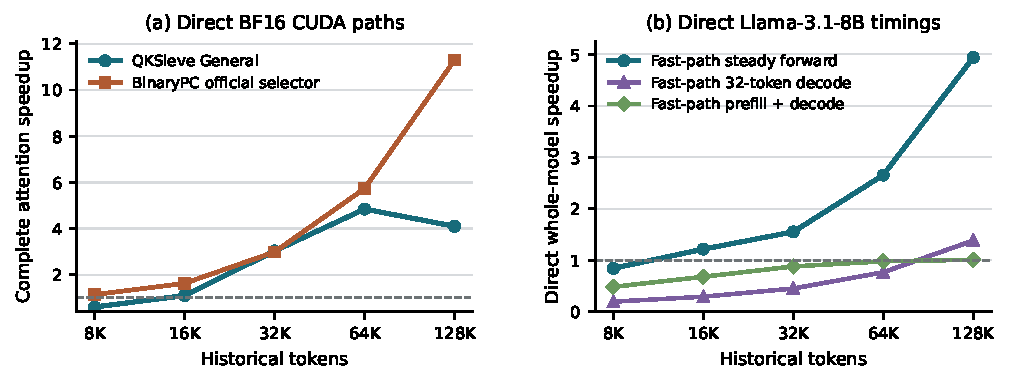
\includegraphics[width=\linewidth]{figures/qksieve_system_diagnostics.pdf}
  \caption{Direct RTX~3090 measurements.  Left: complete BF16 single-layer
  attention calls for General and the released BinaryPC selector.  Right:
  Fast-path Llama-3.1-8B steady forwards, measured 32-token decode intervals,
  and prefill-plus-decode requests; the right panel is a crossover diagnostic,
  not a General-profile speed claim.  No curve is reconstructed from a sum of
  independently timed stages.}
  \label{fig:speed}
\end{figure}

\begin{table}[!htbp]
\caption{Frozen native-MHA FP16 component timings on RTX~3090.  Components
are invoked independently to locate bottlenecks and are not summed to
reconstruct the directly timed complete path.}
\label{tab:deployment-breakdown}
\centering
\begin{tabular}{rrrrr}
\toprule
Length & Query prepare & Selector scan & Sparse attention & Complete path \\
\midrule
8K & .0336 & .0365 & .0438 & .1386 \\
16K & .0335 & .0468 & .0910 & .1946 \\
32K & .0299 & .0634 & .1107 & .2312 \\
64K & .0302 & .0999 & .1186 & .2684 \\
128K & .0303 & .1673 & .1630 & .3810 \\
\bottomrule
\end{tabular}
\end{table}

Query preparation is nearly length-independent.  The packed scan and exact
sparse consumer dominate at 128K, while candidate materialization, gather,
and launch overhead explain the gap between the independent stages and the
complete call.  Capping quantile samples at 512 specifically reduces the
long-context selector term; it does not change the linear packed-index scan.

\begin{table}[!htbp]
\caption{Earlier GQA-4 BF16 QKSieve Fast--Robust timing on RTX~3090.  Complete paths
are timed directly; scan and consumer rows are independently invoked
diagnostics and are not added.  Robust uses rank-16 block-affine INT4 Value
coefficients and $\alpha=.5$.}
\label{tab:robust-direct-timing}
\centering
\begin{tabular}{lrr}
\toprule
Direct operation, 128K & Time (ms) & Speed vs Full \\
\midrule
Full attention & 2.451 & 1.000$\times$ \\
Fast complete attention & .398 & 6.161$\times$ \\
Robust complete attention & .595 & 4.119$\times$ \\
General conditional complete call & .598 & 4.100$\times$ \\
Robust Key+Value-tail scan & .347 & -- \\
Robust exact-selected-plus-tail consumer & .190 & -- \\
\bottomrule
\end{tabular}
\end{table}

The Robust per-token index contains 240 Key bits, 64 Value coefficient bits,
and two amortized block-metadata bits, totaling 7.471\% of FP16 K+V.  Its
12-case whole-model geometric-mean steady speedup is 3.224$\times$; one-time
initialization amortized over 64 measured decode tokens gives 1.125$\times$.
These values are lower than Fast but pair with the independently validated
native-128K robustness result.

\begin{table}[!htbp]
\caption{Long-history physical CUDA attention scaling with a fixed
1,280-token exact-attention budget.  The 256K/512K rows sum 36 Qwen3-style
layers and exclude non-attention model work and first index construction.
The strict 256K diagnostic rejects this budget as quality-valid, and
Qwen3-4B does not natively support 512K quality; these rows therefore isolate
low-budget operator scaling.}
\label{tab:long-history-attention}
\centering
\begin{tabular}{lrrr}
\toprule
History & Full SDPA & \method & Speedup \\
\midrule
128K, one layer & 2.439 ms & .360 ms & 6.78$\times$ \\
256K, $B=1280$ & 175.008 ms & 12.650 ms & 13.83$\times$ \\
512K, $B=1280$ & 380.282 ms & 17.513 ms & 21.71$\times$ \\
\bottomrule
\end{tabular}
\end{table}

\begin{table}[!htbp]
\caption{High-fidelity long-history attention timing on one RTX~3090.
\method uses 24\% active tokens and includes Query projection/quantization,
low-bit retrieval, sampled-quantile selection, and exact sparse attention.
The pre-expanded baseline excludes GQA replication, whereas the HF-style
baseline includes \texttt{repeat\_kv} and SDPA.  Times sum 36 Qwen3-style
layers and exclude index construction and non-attention model work.}
\label{tab:long-history-highfidelity-attention}
\centering
\small
\resizebox{\linewidth}{!}{%
\begin{tabular}{lrrrrr}
\toprule
History & Pre-expanded SDPA & HF GQA+SDPA & \method & vs.\ pre-expanded &
vs.\ HF \\
\midrule
256K & 175.104 ms & 567.610 ms & 199.992 ms & .876$\times$ &
2.838$\times$ \\
512K & 348.520 ms & 1135.721 ms & 373.800 ms & .932$\times$ &
3.038$\times$ \\
\bottomrule
\end{tabular}}
\end{table}

Thus the high-fidelity sparse path is not faster than an idealized SDPA
consumer whose GQA K/V have already been materialized.  Its practical
advantage is relative to the actual HF execution path that performs GQA
replication at every decode step.  We report both denominators rather than
folding replication into an unspecified ``attention overhead.''  At 512K,
the 24\% selector uses 768 stratified samples ($c=128$) so that its confidence
capacity remains within the 16-way ragged-kernel limit.

An old 262,144-token-history plus 16-target stress test gives
Full/\method PPL 5.7518/5.1052 and 100\% top-1 agreement, but those target
positions exceed the declared model limit and are not a native-context
quality claim.  The registered native-boundary rerun instead uses 262,080
history plus 64 targets.  A 524,256-token Full prefill does complete on seven
RTX~3090 GPUs with 22.70 GiB peak allocated and 24.00 GiB peak reserved on
the busiest device.  However, Qwen3-4B has neither native positions nor RoPE
scaling beyond 262,144 tokens, and its extrapolated Full PPL on the diagnostic
window is 5510.6.  We therefore use 512K only to measure relative
Full--sparse approximation and system stress, not native task quality.

\begin{table}[!htbp]
\caption{Strict native-boundary 256K causal-PPL frontier over four
independently shuffled 20-Newsgroups windows (262,080 history plus 64 targets
per window; 256 paired target tokens).  Retention is computed from pooled
NLL differences.  The interval bootstraps the four windows as clusters and
is therefore diagnostic rather than a final cross-corpus confidence claim.}
\label{tab:256k-frontier}
\centering
\small
\resizebox{\linewidth}{!}{%
\begin{tabular}{rrrrr@{\qquad}r}
\toprule
Active & Retention (95\% CI) & Top-1 & KL & Steady & Online \\
\midrule
7.977\% & 94.440\% [93.38, 95.68] & 78.516\% & .04365 &
5.511$\times$ & 4.925$\times$ \\
9.977\% & 96.260\% [94.53, 97.73] & 82.031\% & .03266 &
5.345$\times$ & 5.097$\times$ \\
11.927\% & 96.949\% [94.79, 98.43] & 83.984\% & .02696 &
4.453$\times$ & 4.283$\times$ \\
15.951\% & 97.418\% [95.43, 99.07] & 83.594\% & .02250 &
3.642$\times$ & 3.377$\times$ \\
20.055\% & 99.072\% [97.62, 100.55] & 84.766\% & .01349 &
2.959$\times$ & 2.887$\times$ \\
\textbf{23.958\%} & \textbf{100.250\% [99.40, 101.06]} &
\textbf{92.188\%} & \textbf{.00733} & \textbf{2.989$\times$} &
\textbf{2.911$\times$} \\
\bottomrule
\end{tabular}}
\end{table}

The 23.958\% point statistically matches Full on these windows; retention
slightly above 100\% is not evidence that sparse attention generally improves
the model.  Averaged over the four runs, Full and \method steady decode are
588.942 and 197.019 ms/token, respectively.  Common prefill is 1058.826 s,
so request-level speedup reaches $2\times$ only after approximately 5,436
generated tokens.  The complete FP16 K/V remain GPU-resident: ``Active''
denotes exact-attention compute, not cache-memory retention.

\begin{table}[!htbp]
\caption{Strict-256K oracle budget diagnosis on the same four windows and
256 paired target tokens as \cref{tab:256k-frontier}.  Exact-QK computes
all historical FP16 QK scores before selecting the stated budget; the
low-bit proxy uses the frozen QK-balanced/Key-MSE 240-bit index and complete
proxy top-$k$.  Both consumers use exact attention over original FP16 K/V.}
\label{tab:256k-oracle-gap}
\centering
\small
\resizebox{\linewidth}{!}{%
\begin{tabular}{lrrrrrr}
\toprule
Selector & Exact/head & Active & Oracle mass & Retention (95\% CI) & Top-1 & KL \\
\midrule
Exact FP16 QK & 1,280 & .488\% & 90.002\% &
\textbf{100.240\% [99.48, 100.88]} & 90.625\% & \textbf{.00516} \\
Exact FP16 QK & 2,560 & .977\% & 93.057\% &
\textbf{100.148\% [99.54, 100.68]} & 92.969\% & \textbf{.00297} \\
Low-bit proxy & 1,280 & .488\% & -- &
80.771\% [77.84, 83.92] & 67.188\% & .24246 \\
Low-bit proxy & 2,560 & .977\% & -- &
86.132\% [84.68, 87.77] & 71.094\% & .15092 \\
\bottomrule
\end{tabular}}
\end{table}

\begin{table}[!htbp]
\caption{Matched 128K--256K selector crossover.  Both lengths use the same
frozen QK-balanced/Key-MSE template, complete proxy top-$k$, four text
windows and seeds, and 256 paired targets.  Entries are PPL retention with
four-window cluster-bootstrap 95\% intervals.}
\label{tab:128k-256k-selector-crossover}
\centering
\small
\resizebox{\linewidth}{!}{%
\begin{tabular}{lrrrr}
\toprule
History & Exact-1,280 & Proxy-1,280 & Exact-2,560 & Proxy-2,560 \\
\midrule
128K & 100.805\% [99.40, 102.23] & 98.993\% [96.53, 102.99] &
100.345\% [99.14, 101.57] & 100.005\% [97.66, 103.02] \\
256K & 100.240\% [99.48, 100.88] & 80.771\% [77.84, 83.92] &
100.148\% [99.54, 100.68] & 86.132\% [84.68, 87.77] \\
\bottomrule
\end{tabular}}
\end{table}

\begin{table}[!htbp]
\caption{Strict-256K coordinate--allocation split at top-1,280.  All rows
use the same four windows, 256 paired targets, complete top-$k$, and exact
attention over original FP16 K/V.  Online decode amortizes one-time selector
preparation over approximately 63 timed steps and excludes common prefill.}
\label{tab:256k-selector-cause}
\centering
\small
\resizebox{\linewidth}{!}{%
\begin{tabular}{lrrrrr}
\toprule
Selector/index policy & Retention (95\% CI) & Top-1 & KL & Steady & Online \\
\midrule
Exact FP16 QK & 100.240\% [99.48, 100.88] & 90.625\% & .00516 & -- & -- \\
Frozen coord./frozen bits & 80.771\% [77.84, 83.92] & 67.188\% & .24246 &
7.785$\times$ & 6.668$\times$ \\
Frozen coord./local bits & 89.911\% [84.13, 94.28] & 77.344\% & .13332 &
7.766$\times$ & 5.259$\times$ \\
Local coord./fixed bits & \textbf{100.443\% [99.80, 101.02]} & 91.016\% &
.00620 & 7.671$\times$ & \textbf{4.955$\times$} \\
Local coord./local bits & 100.430\% [99.78, 100.99] & 91.016\% &
.00622 & \textbf{7.733$\times$} & 4.055$\times$ \\
Frozen all-INT8 & 100.267\% [99.48, 100.91] & 91.016\% & \textbf{.00508} &
1.882$\times$ & 1.846$\times$ \\
\bottomrule
\end{tabular}}
\end{table}

\begin{figure}[!htbp]
\centering
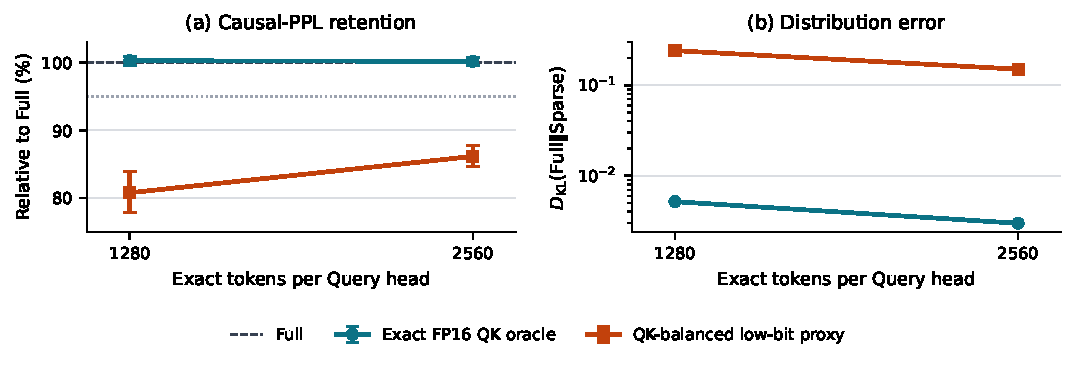
\includegraphics[width=.78\linewidth]{figures/qksieve_256k_oracle_gap.pdf}
\caption{At the native 256K boundary, 1,280 exact tokens per Query head are
already sufficient when selected by Exact FP16 QK.  Doubling the low-bit
proxy budget improves quality but leaves a large selection gap.  Error bars
are four-window cluster-bootstrap 95\% intervals.}
\label{fig:256k-oracle-gap}
\end{figure}

This control reverses the initial fixed-budget diagnosis.  Exact-QK
top-1,280 retains 100.24\% PPL with KL .0052 at only .488\% active, whereas
the frozen low-bit proxy retains 80.77\%; proxy top-2,560 reaches 86.13\%.
Under the matched 128K protocol, the same proxy retains 98.99\% and
100.01\%, respectively (\cref{tab:128k-256k-selector-crossover}).
Thus the 23.958\% point in \cref{tab:256k-frontier} compensates proxy
misranking rather than a fundamental attention budget.  The orthogonal split
in \cref{tab:256k-selector-cause} localizes the cause.  Reallocating the same
240 bits under frozen coordinates recovers only 89.91\%, whereas local
coordinates with fixed 4-1-1-1-1-1-0-0 bits recover 100.44\%, statistically
matching local coordinates plus local allocation (100.43\%).  Coordinate
shift is therefore dominant in this stress test; dynamic bits are neither
necessary nor measurably beneficial here.  Local fixed bits retain
7.67$\times$ steady and 4.96$\times$ 64-token online whole-model speed,
while frozen all-INT8 confirms that more precision can mask stale
coordinates at much lower speed.  We omit oracle speed because its dense
FP16 QK scan is diagnostic, not deployable.

\begin{table}[!htbp]
\caption{Qwen3-4B 512K extrapolation stress on one 20-Newsgroups causal-PPL
window (524,256 history plus 32 targets).  The absolute Full PPL is 5510.6;
retention therefore measures only proximity to the same extrapolated Full
distribution.  Online decode amortizes selector setup over the 31 timed
steps and excludes the common 4,297--4,299 s prefill.}
\label{tab:512k-extrap-frontier}
\centering
\small
\begin{tabular}{rrrrrrr}
\toprule
Active & Retention & Top-1 & KL & Steady & Online & Count range \\
\midrule
2.951\% & 105.34\% & 93.75\% & .0978 & 10.70$\times$ & 9.00$\times$ &
5,117--33,365 \\
3.947\% & 101.63\% & 96.88\% & .0794 & 10.72$\times$ & 8.13$\times$ &
6,999--48,828 \\
4.880\% & 99.97\% & 93.75\% & .0754 & 8.98$\times$ & 7.82$\times$ &
8,805--49,759 \\
5.872\% & 98.57\% & 96.88\% & .0592 & 7.72$\times$ & 6.85$\times$ &
11,359--66,293 \\
\bottomrule
\end{tabular}
\end{table}

\begin{table}[!htbp]
\caption{Matched LongBench selector screening on 160 strict Llama-3.1-8B
pairs (10 examples per task).  Every sparse row uses the same active-token
schedule and original-KV consumer.  FIER, Quest, RaBitQ, and SparQ rows are
audited formula/reference controls, not official optimized-system timings.}
\label{tab:baseline-placeholder}
\centering
\small
\begin{tabular}{lrrr}
\toprule
Method & Index bits/token/KV-head & Active & Full-relative quality \\
\midrule
Full & 0 & 100.00\% & 100.000\% \\
\method reference & 240 & 7.440\% & 99.789\% \\
FIER RTN-1 g32 reference & 256 & 7.440\% & 100.010\% \\
Quest-P16, page-rounded & 256 & 7.562\% & 92.217\% \\
RaBitQ RTN-1 reference & 224 & 7.440\% & 100.012\% \\
SparQ-R32 selector only & 0 & 7.440\% & 99.623\% \\
SparQ-R32 complete formula & 0 & 7.440\% & 99.950\% \\
UNIQUE-P8 equation reference & 258 & 7.494\% & 93.193\% \\
\bottomrule
\end{tabular}
\end{table}

\begin{table}[!htbp]
\caption{Released BinaryPC comparison.  Quality uses 160 strict LongBench
pairs (ten examples per task) and remains too small for a superiority claim.
Speed uses direct BF16 single-layer CUDA calls at 128K with the same $B(N)$
and exact sparse consumer; \method speed is its deployment selector, whereas
quality is its deterministic reference selector.}
\label{tab:binarypc-public-comparison}
\centering
\begin{tabular}{lrrrr}
\toprule
Method & Index bits & Active & Full-relative quality & 128K attention \\
\midrule
Full & 0 & 100.00\% & 100.000\% & 1.000$\times$ \\
BinaryPC released & 64 & 7.440\% & 99.250\% & 11.295$\times$ \\
\method & 240 & 7.440\% & 99.789\% & 6.798$\times$ \\
\bottomrule
\end{tabular}
\end{table}

The FIER row is a strict same-sample, same-budget reference-quality run; its
quality harness is not used for latency.  The Quest-P16 control stores
per-page extrema and loads complete 16-token pages.  The SparQ complete
formula adds its $r=32$ temperature, local window,
approximate selected mass, and running mean-Value correction.  The official
RaBitQCache efficiency artifact requires CUDA~12.8 and a modified vLLM; this
RTX~3090 environment uses an older PyTorch CUDA runtime, so we do not report a
fabricated native RaBitQ speed.  The current public Microsoft repository
provides RetroInfer, not a runnable artifact of original RetrievalAttention.


\clearpage
\section{Completed Llama-3.1-8B LongBench Results}
\label{app:longbench}

\begin{table}[h]
\caption{Complete 3,750-pair Llama-3.1-8B LongBench evaluation.
The run uses the frozen auto+plain+full-topk path and official middle
truncation.}
\centering
\resizebox{\linewidth}{!}{
\begin{tabular}{lrrrr}
\toprule
Task & Samples & Full & \method & Relative \\
\midrule
2WikiMQA & 200 & .473495 & .475662 & 100.458\% \\
GovReport & 200 & .337627 & .334587 & 99.100\% \\
HotpotQA & 200 & .486550 & .492022 & 101.125\% \\
LCC & 500 & .631943 & .635199 & 100.515\% \\
MultiNews & 200 & .269995 & .269824 & 99.937\% \\
MultiFieldQA-en & 150 & .562466 & .561067 & 99.751\% \\
Musique & 200 & .273163 & .268762 & 98.389\% \\
NarrativeQA & 200 & .242717 & .237154 & 97.708\% \\
PassageCount & 200 & .099083 & .099583 & 100.505\% \\
PassageRetrieval-en & 200 & .685000 & .685000 & 100.000\% \\
Qasper & 200 & .457071 & .446171 & 97.615\% \\
QMSum & 200 & .232550 & .230128 & 98.958\% \\
RepoBench-P & 500 & .545507 & .548896 & 100.621\% \\
SAMSum & 200 & .443306 & .444600 & 100.292\% \\
TREC & 200 & .695000 & .690000 & 99.281\% \\
TriviaQA & 200 & .914896 & .922980 & 100.884\% \\
\midrule
Macro & 3,750 & .459398 & .458852 & 99.881\% \\
\bottomrule
\end{tabular}}
\end{table}

Seven tasks improve over Full and PassageRetrieval-en ties.  The largest
relative degradations are Qasper (97.615\%), NarrativeQA (97.708\%), and
Musique (98.389\%); no task falls below 97.6\% retention.  The
task-stratified paired-bootstrap 95\% intervals are
[$-.002647$, $.001591$] for the macro-score difference and
[99.424\%, 100.347\%] for retention.  The finalizer verifies 7,500 CSV rows,
3,750 strict pairs, 16 tasks, frozen-path execution fields, prompt limits,
and source hashes.

\clearpage
\section{Required Final Experiments}
\label{app:missing}

\begin{table}[h]
\caption{Quality closure.  ``Pass'' values are pre-registered targets, not
measured results.}
\centering
\resizebox{\linewidth}{!}{
\begin{tabular}{llll}
\toprule
Experiment & Models & Required report & Target \\
\midrule
LongBench 16-task & 2 remaining & Per task, macro, paired CI &
$\ge99\%$ macro \\
RULER 4K--128K & 3 & Per task and length & No unexplained collapse \\
PPL 16K--128K & 3 & Per window, aggregate CI & $\ge99\%$ at 128K \\
Long output & 3 & 1K/2K/4K tokens & Stable retention \\
Multi-turn & 3 & Turn-wise Query drift & Stable retention \\
\bottomrule
\end{tabular}
}
\end{table}

\subsection{Persistent-KV workload contract and measured audit}
\label{app:persistent-kv-todo}

The intended deployment is repeated decoding over a materialized long-context
KV cache, as in multi-turn agents, shared-prefix rollouts, and repeated queries
over a common memory.  This does not remove prefill from accounting: it changes
whether prefill and index construction are paid once or once per decode.  The
final submission must populate the following timing contracts independently;
numbers from one row cannot be used to fill another.

\begin{table}[h]
\caption{Persistent-KV timing contracts.  The current 32/64K audit instantiates
all rows within one request-local QK basis; H100, 128K, and cross-prompt Query
drift remain preregistered.}
\label{tab:persistent-kv-todo}
\centering
\resizebox{\linewidth}{!}{
\begin{tabular}{llll}
\toprule
Contract & Included interval & Intended use & Required report \\
\midrule
Cold single-use & Dense prefill + index build + $G$ decode & One-shot request & E2E, TTFT, TPOT \\
Warm persistent & Query setup + $G$ decode; KV/index resident & Cached-prefix query & E2E, first token, TPOT \\
Shared-prefix reuse & One prefill/index shared by $R$ branches & Agent rollouts & Amortized latency, throughput, break-even \\
Append-only turn & Delta prefill + delta index append + decode & Multi-turn agent & Append cost, TPOT, turn-wise quality \\
\bottomrule
\end{tabular}}
\end{table}

The current directly timed results are in \cref{tab:persistent-kv-main}.  For
32/64K, the matched Full/QKSieve cold latencies are
83.926/119.551 and 145.195/129.108 ms/token; warm latencies are
83.714/63.347 and 144.910/65.256 ms/token; four-branch amortized latencies are
83.762/77.399 and 144.971/81.204 ms/token; append-only latencies are
83.874/63.611 and 145.012/65.597 ms/token.  These are one-seed RTX~3090
measurements and exclude the dense prefill shared by both methods.

The audit independently reparses every layer rather than trusting a benchmark
success flag.  It verifies 32 populated Key and Value indices, six snapshots,
five rewinds, stable storage pointers and rebuild counters, deterministic
branch replay, and exactly one token of deferred index append after decode.
The branch test keeps the request-local QK basis fixed.  A semantically new
prompt that changes Query statistics is outside this reuse claim and must pay
for a new request-local transform and index.

Let $P$ be the shared dense-prefill cost, $I$ the one-time persistent-index
construction cost, $H_f$ and $H_s$ the per-request dense and sparse setup
costs, $D_f$ and $D_s$ their measured per-token decode costs, and $A$ the
total incremental append cost.  For $R$ reuses that each generate $G$ tokens,
the registered accounting is
\begin{align}
T_{\mathrm{full}} &= P + R(H_f + G D_f), \\
T_{\mathrm{QKSieve}} &= P + I + R(H_s + G D_s) + A.
\end{align}
The measured break-even boundary must therefore satisfy
\begin{equation}
R G(D_f-D_s) > I + R(H_s-H_f) + A,
\label{eq:persistent-break-even}
\end{equation}
rather than being inferred from steady-state attention speed alone.

The evaluation grid is $N\in\{16,32,64,128\}$K,
$G\in\{32,64,256,1024\}$, and $R\in\{1,2,4,8,16,32\}$ on repeated-query,
append-only dialogue, and branching-rollout traces.  It reports latency,
throughput, peak memory, index bytes, active KV, and quality retention for
every cell.  Resident-cache timing excludes cache lookup only when that lookup
is identical for Full and \method; eviction or reload costs are reported
separately.

Before any warm or reuse result is admissible, the implementation must pass a
cache-lifecycle audit: the auxiliary index is constructed once and persists
with the exact KV; an unchanged historical prefix is never reprojected or
requantized at a request boundary; newly appended tokens incur only incremental
index maintenance; and all per-request Query preparation is inside the timed
interval.  A request-local basis that re-encodes historical Keys cannot fill
the warm rows.  Reusing the index does not permit temporal reuse of old
candidates, a learned router, or Full-attention fallback.

\begin{table}[h]
\caption{Required method and systems comparisons.}
\centering
\resizebox{\linewidth}{!}{
\begin{tabular}{lll}
\toprule
Group & Variants & Matching rule \\
\midrule
Closest baseline & FIER 1-bit, \method & Index bytes and active tokens \\
Selector quality & Quest-P16, SparQ-R32 selector/formula, \method & Active-token policy and exact-KV consumer \\
Native systems & Quest, SparQ, RetroInfer & Model, hardware, and complete system \\
Paper reported & RetrievalAttention & Model and operating point from paper \\
Coordinates & Key-PCA, random rotation, QK-balanced & Index bytes \\
Rate & Uniform, fixed 4-4-2-1, automatic & 240 bits \\
Query estimate & 1/4/8/16/32 positions; templates & Frozen settings \\
Shrinkage & $0,.25,.5,.75,.9$ & Held-out traces \\
Systems & 16K/32K/64K/128K & 64/256/1,024 output \\
\bottomrule
\end{tabular}}
\end{table}

For the Query-estimate rows, the production transform and allocation use the
last eight prompt positions even when the trace records a 32-position tail.
We report moment operator-norm error, singular gaps and subspace angles at
all 16-D band boundaries, held-out allocation regret, centered score RMSE,
top-$2\%$ recall, and oracle/proxy omitted mass by generation-position
bucket.  Natural-EOS and teacher-forced continuation traces are separate
artifacts.  Long-output coverage is accepted only when the registered
1K/2K/4K Query was actually captured.

Every systems row must include index build, per-token index append, Query
projection, low-bit scan, top-$k$, gather, exact sparse attention, remaining
model time, total decode, request latency, peak GPU memory, and the
no-attention Amdahl ceiling.
FIER must be run from its official implementation or an audited faithful port;
formula-level trace simulations are labeled mechanism studies only.
The Quest selector control reports page-rounded loaded tokens.  The
selector-only SparQ control excludes the mean-Value correction.  A separate
matched-budget formula reference includes SparQ's temperature, local mask,
selected-mass estimate, and running mean-Value correction, but remains a
reference PyTorch path and cannot be presented as the optimized official SparQ
system.  The current public Microsoft repository implements RetroInfer; it is
reproduced as a separate CPU--GPU native system, while original
RetrievalAttention numbers remain explicitly paper reported.  Neither
heterogeneous system is described as index-byte matched to a GPU-resident
method.
Before any final quality and speed numbers are combined, the artifact
verifier checks the frozen method contract, current source hashes, strict
sample pairing, model/task coverage, length/output grid, and peak-memory
fields.  A missing artifact is a failed gate rather than an implicit pass.
